%*******************************************************************************
%****************************** Chapter Five ***********************************
%*******************************************************************************

\chapter{Clustering Gene Expression Data}\label{ch:Clustering_Gene_Expression_Data}

\ifpdf
    \graphicspath{{Chapter5/Figs/Raster/}{Chapter5/Figs/PDF/}{Chapter5/Figs/}}
\else
    \graphicspath{{Chapter5/Figs/Vector/}{Chapter5/Figs/}}
\fi
%\title{Increasing Power by Sharing Information from Genetic Background and Treatment in Clustering of Gene Expression Time Series}

%\section{Introduction}
The dynamic behaviour or analysis of time series data in particular clusters is important for exploring and understanding gene networks. In many conventional time series models, one key requirement is data with regular intervals. Gene expression experiments data with regular intervals might be less informative or may not be optimal from a statistical perspective or even may not be cost effective for various reasons. A model designed to obtain data with regular intervals may not elicit as much information as a method designed to collect pertinent special temporal features. Again, in many cases multiple biological replicates are available when the same experiments are repeated multiple times. For these cases simply considering only one experiment or taking the mean values from different replicates may not be the best solution. Interesting information might be discarded while dealing only with one data set or with their mean values.

The aim of this chapter is to specify the significantly different genes that may effect the speed of ALS progression by building a new model. We used Gaussian processes and here we introduce  \emph{coregionalization} principle while developing the kernel of the Bayesian hierarchical Gaussian process model. We believe, there might be some degree of temporal continuity between different replicates, conditions and/or genetic backgrounds. So, the kernel designed considering \emph{coregionalization} model will consider the shared information between those replicates and conditions of genetic background. We used $python$ programming language based tool $GPy$(The GPy \cite{gpy2014}), to develop our model. Later we optimized these models and compared them based on likelihood scores and select the best. %\footnote{\url{http://sheffieldml.github.io/GPy/}}

Amyotrophic lateral sclerosis (ALS) is a diverse neurodegenerative disorder with around 10\% of familial cases and the remaining sporadic. The disease is currently irreversible from onset and heterogeneous with variable severity in terms of speed of progression of the disease course. Injury and cell death of motor neurons in the brainstem, spinal cord and motor cortex are the main reasons of this relentlessly progressive disorder (\cite{Brockington:2013, Ferraiuolo:2011, Haverkamp:1995, Peviani:2010}). Among the familial ALS [fALS] 20\% is caused by mutation in the $Cu/Zn$ $Superoxide$ $Dismutase 1$ $(SOD1)$ gene. The median survival of this lethal disorder is less than 5 years, only 20\% patients live longer than 5 years and less than 10\% patients survive more than 10 years from the symptom onset (\cite{Beghi:2011, Saccon:2013}). The speed of disease progression is not clear from the biological basis. Even in fALS, affected members clearly show the clinical heterogeneity in terms of site of onset, age and progression rate of the disease. In a study, \cite{Camu:1999} reported the presence of potential gene modifiers and pathways that particularly affect the disease phenotype. Mutation in the $SOD1$ gene notably characterized the distinctive nature by intrafamilial and interfamilial variabilities in the phenotype. Many of the clinical and pathological features of human ALS can be replicated very well by transgenic mice. These murine models also mimic the human disease and show the heterogeneity in the disease progression for the clinical phenotype. These variability may be related with expression levels of mutant $SOD1$ protein or specific $SOD1$ mutations (\cite{Turner:2008}).

In a study \cite{Pizzasegola:2009} reported that disease progression is much faster in $129Sv$ mice with the survival time of $129\pm5$ days, while the $C57$ mouse strain can survive $180\pm16$ days. Both the $129Sv$ and $C57$ carry the same copy numbers of human mutant $SOD1$ and express the same amount of mutant $SOD1^{G93A}$ messenger RNA in the spinal cord.  \cite{Marino:2015} reported about the differences in protein quality control of these mouse models in terms of speed of progression of the disease course.

Here in this work, we built a mathematical model to cluster gene expression time series data using hierarchical Gaussian process. Then as a part of validation we performed investigation of these clusters. We have calculated the enrichment scores (\cite{Huang:2007, Huang:2009Enrichment}) for every cluster using $DAVID$\footnote{\url{http://david.abcc.ncifcrf.gov/tools.jsp}} (Database for Annotation, Visualization and Integrated Discovery) (\cite{Huang:2009David}) and identified clusters which have very high enrichment scores.  We carried out further analysis of clusters with high enrichment score and which also demonstrated some interesting characteristics in their dynamic behaviour at the four time stages (pre-symptom, onset, symptom and end-stage) of disease course. Our functional annotation clustering and pathway analysis reveal some interesting information for a group of genes which might have some functionality for the speed of propagation of ALS particularly with reference to this specific type of mouse model. 

\section{Related work}
Gene expression time series data has been used extensively over the last few decades and implemented for \textit {in-silico} experiments to investigate various fundamental biological processes. Among the many processes examined, some of the notable examples are cell cycle \cite{Spellman:1998}, cell signalling \cite{Barenco:2006}, regulatory activity \cite{Sanguinetti:2006}, and developmental process \cite{Tomancak:2002}. Gaussian processes have been applied to gene expression time series widely with several aims and analyses, such as transcription factor target identification (\cite{Honkela:2010}), inference of RNA Polymerase transcription dynamics (\cite{Maina:2014}), and ranking differentially expressed time series (\cite{Kalaitzis:2011}).

Hierarchical models can significantly improve the inference in the Bayesian statistical problems (\cite{Gelman:2004}) while dealing with multiple related groups of data allowing exchange of information. Inference on the whole structure of data is always preferable than partial independent structure. Estimating replicate time shifts were proposed by \cite{Liu:2010}, where they used Gaussian process regression with uncertain measurement of mRNA expression. This method require a large number of variables optimization. Previously, \cite{Ng:2006} also \cite{Medvedovic:2004} used clustering method to model replicates using hierarchical structure. Both of the model compute the replicate variance as multivariate Gaussian around some gene-specific mean.

In a clustering application Gaussian process regression could be useful for parsimonious temporal inference. Temporal covariance of genes within a cluster can be designed by adding a hierarchical layer, again covariance between multiple biological replicates can be constructed considering one more hierarchical layer (\cite{Menzefricke:2000, Hensman:2013}). Whilst Gaussian process also overcome the requirement of evenly spaced time points for time expression data.

Here we constructed a hierarchical Gaussian process (\cite{Hensman:2013}) based model to analyse the gene expression time series data collected from four mouse models with different genetic background ($129Sv$ and $C57$ with transgenic and non-transgenic). We also considered their replicates (four in our case) and build a covariance matrix based on their shared information and the time points were pre-symptom, onset, symptom and end stage of the disease course.


\section{Methodology}

% % \subsection{Gaussian Process definition}
% % A Gaussian process is a collection of random variables, any finite number of which have a 
% % joint Gaussian distribution \cite{Rasmussen_and_Williams:2006}. It is a continuous
% % stochastic process and defines probability distributions for functions. It can be also view
% % as set of random variables indexed by a continuous variable: $ f(\textbf{x})$ chosen from a random
% % function variables $ \textbf{f} = \{ f_1, f_2, f_3,..., f_N\}$, with corresponding indexed inputs
% % $ \textbf{X} = \{ \textbf{x}_1, \textbf{x}_2, \textbf{x}_3,..., \textbf{x}_N\}$. In Gaussian processes,
% % variables from these random functions are normally distributed and as a whole can be represented as a
% % multivariate Gaussian distribution
% % \begin{equation} \label{eq:2.2}
% % p(\textbf{f}|\textbf{X})= \mathcal{N}(\boldsymbol\mu,\textbf{K}),
% % \end{equation}
% % where $\boldsymbol\mu$ is the mean and $\textbf{K}$ is covariance of Gaussian distribution
% % $\mathcal{N}(\boldsymbol\mu,\textbf{K})$.
% % The Gaussian distribution is over vectors but the Gaussian process is over functions.
% % 
% % If $f(\textbf{x})$ is a real process, a Gaussian process is completely defined by its mean function
% % and covariance function given in equation \ref{eq:2.3} and equation \ref{eq:2.4} respectively.
% % Usually, the $m(\textbf{x})$  and the covariance function $k(\textbf{x},\textbf{x\textprime})$
% % are defined as-
% % \begin{equation} \label{eq:2.3}
% % m(\textbf{x})= \mathbb{E}[f(\textbf{x})],
% % \end{equation}
% % \begin{equation} \label{eq:2.4}
% % k(\textbf{x},\textbf{x\textprime})= 
% % \mathbb{E}[(f(\textbf{x})-m(\textbf{x}))(f(\textbf{x}\textprime)-m(\textbf{x}\textprime))],
% % \end{equation}
% % where $\mathbb{E}$ represents the expected value.
% % We denote the Gaussian process as-
% % \begin{equation} \label{eq:GP}
% % f\left(\textbf{x} \right)\sim \mathcal{GP} \left(m \left(\textbf{x}\right), k \left(\textbf{x},\textbf{x\textprime}\right) \right).
% % \end{equation}
% % 
% % The covariance matrix $\textbf{K}$ is constructed from the covariance function
% % $k(\textbf{x},\textbf{x\textprime})$ and 
% % $\textbf{K}_{ij}=k(\textbf{x}_i,\textbf{x}_j)$.
% % 
% % 
% % \subsection{Gaussian Process Regression}
% % Gaussian process regression can be done using the marginal and conditional properties of multivariate
% % Gaussian distribution. Let's consider that we have some observations $\mathbf{f}$ of a function at observation
% % point $\mathbf{x}$. Now we wish to predict the values of that function at observation points $\mathbf{x_\star}$,
% % which we are representing by $\mathbf{f_\star}$. Then the joint probability of $\mathbf{f}$ and $\mathbf{f_\star}$
% % can be obtained from
% % \begin{equation} \label{eq:jointPro_f_f*}
% % p \left( \begin{bmatrix} \mathbf{f} \\\mathbf{f_\star} \end{bmatrix} \right) =
% % \mathcal{N}\left( \begin{bmatrix} \mathbf{f} \\\mathbf{f_\star} \end{bmatrix} \middle|
% % \mathbf{0}, \begin{bmatrix} \mathbf{K_{x,x}} & \mathbf{K_{x,x_\star}} \\
% % 			    \mathbf{K_{x_\star,x}} & \mathbf{K_{x_\star,x_\star}} \end{bmatrix} \right)
% % \end{equation}
% % where the covariance matrix $ \mathbf{K_{x,x}}$ has elements derived from the covariance function 
% % $ k \left(x,x\textprime \right)$, such that the $ \left(i,j \right)^{th}$ element of $ \mathbf{K_{x,x}}$ is
% % given by $k \left( \mathbf{x} \left[ i\right],\mathbf{x} \left[ j\right] \right) $ 
% % The conditional property of a multivariate Gaussian is used to perform regression the. The conditional
% % property can be represented by
% % \begin{equation} \label{eq:condProMvG}
% % p \left( \mathbf{f} \middle| \mathbf{f_\star} \right) =
% % \mathcal{N}\left( \mathbf{f_\star} \middle| \mathbf{K_{x_\star,x}}  \mathbf{K^{-1}_{x,x}} \mathbf{f,} \mathbf{K_{x_\star,x_\star}} - 
% % \mathbf{K_{x_\star,x}} \mathbf{K^{-1}_{x,x}} \mathbf{K_{x,x_\star}}\right).
% % \end{equation}
% % 
% % In ideal case the observations $\mathbf{f}$ is noise free but in practice it is always corrupted with some noise.
% % Let's consider $\mathbf{y}$ is the corrupted version of $\mathbf{f}$. If we consider this noise as Gaussian noise
% % then we can write $p \left( \mathbf{y} \middle| \mathbf{f} \right) = \mathcal{N} \left( \mathbf{y} \middle| \mathbf{f},
% % \sigma^2 \mathbf{I} \right) $, where $ \sigma^2 $ is the variance of the noise and $\mathbf{I}$ is the identity
% % matrix with appropriate size and marginalise the observation $\mathbf{f}$. Then the joint probability of 
% % $\mathbf{y}$ and $\mathbf{f_\star}$ can be represented by
% % \begin{equation} \label{eq:jointPro_y_f*}
% % p \left( \begin{bmatrix} \mathbf{y} \\\mathbf{f_\star} \end{bmatrix} \right) =
% % \mathcal{N}\left( \begin{bmatrix} \mathbf{y} \\\mathbf{f_\star} \end{bmatrix} \middle|
% % \mathbf{0}, \begin{bmatrix} \mathbf{K_{x,x}}+ \sigma^2\mathbf{I} & \mathbf{K_{x,x_\star}} \\
% % 			    \mathbf{K_{x_\star,x}} & \mathbf{K_{x_\star,x_\star}} \end{bmatrix} \right).
% % \end{equation}
% % Regression with Gaussian process can be seen as a Bayesian method. From the knowledge of a $prior$ 
% % over a function we proceed to a $posterior$ and this happens in a closed from of equation 
% % \ref{eq:condProMvG}. 
% % 
% % To construct the covariance function still we need to consider the hyperparameters. 
% % The most efficient and commonly used selection technique for hyperparameters in Gaussian process is  
% % maximum likelihood. If we consider all the hyperparameters $\alpha$, $\sigma^2$ and 
% % $l$ in to a vector $\boldsymbol{\theta}$, then we can use gradient methods to optimize
% % $p \left(\mathbf{y}\middle|\boldsymbol{\theta}\right)$ with respect to $\boldsymbol{\theta}$. The log
% % likelihood is given by
% % \begin{equation} \label{eq:Likelihood}
% % \begin{split}
% %  p \left(\mathbf{y}\middle|\boldsymbol{\theta}\right) =  
% %     - \frac{D}{2}\log2\pi & - \frac{1}{2}\times \log \left| \mathbf{K_{x,x}} + \sigma^2\mathbf{I}\right|\\
% %     & - \frac{1}{2}\mathbf{y}^\top \left[\mathbf{K_{x,x}} + \sigma^2\mathbf{I} \right]^{-1}\mathbf{y}.
% % \end{split}
% % \end{equation}
% % 
% % The selection of the hyperparameters $\boldsymbol{\theta}$ can be done using log maximum likelihood, 
% % which is given by
% % \begin{equation} \label{eq:LML}
% %  \boldsymbol{\theta}_{max} = argmax \left( p\left(\mathbf{y}\middle|\boldsymbol{\theta}\right) \right).
% % \end{equation}

\subsection{Hierarchical Gaussian Process}
Our gene expression time series came from four different genetic background or strains and there are four biological replicates. So for every individual gene we can incorporate these in an hierarchical fashion. Let's, the vector of measurements ${\textbf y}^{i}_{nr}$ denotes gene expression of $n^{th}$ gene in the $r^{th}$ biological replicate and $i^{th}$ biological strain or condition. Measurements were made at different times and collected into the vector $\textbf{x}^{i}_{nr}$, where $n, r$ and $i$ represents the same as before. The data for the $n^{th}$ gene and $i^{th}$ strain is denoted by ${\textbf Y}^{i}_n = \{{\textbf y}^{i}_{nr}\}^{R}_{r=1}$ and ${\textbf X}^{i}_n = \{{\textbf x}^{i}_{nr}\}^{R}_{r=1}$, where $R$ is the total number of replicates. The data for the $n^{th}$ gene is represented by ${\textbf Y}_n = \{{\textbf Y}^{i}_{n}\}^{S}_{i=1}$ and ${\textbf X}_n = \{{\textbf X}^{i}_{n}\}^{S}_{i=1}$, where $S$ is the total number of strains or conditions.

Let's consider some underlying function $g_n\left(x\right)$ model gene expression activity of the $n^{th}$ gene, we have other functions $e_{nr}\left(x\right)$ which consider $r^{th}$ replicates and finally we have some other functions $f_{inr}\left(x\right)$ for the $i^{th}$ condition of the genetic background. The Gaussian process models are given by
\begin{equation} \label{eq:hGPn}
g_n\left(x\right) \sim \mathcal{GP} \left(\textbf 0,k_g\left(x,x' \right)\right)
\end{equation}
\begin{equation} \label{eq:hGPnr}
e_{nr}\left(x\right) \sim \mathcal{GP} \left(g_n\left(t\right),k_e\left(x,x' \right)\right)
\end{equation}
\begin{equation} \label{eq:hGPinr}
f_{inr}\left(x\right) \sim \mathcal{GP} \left(e_{nr},k_f\left(x,x' \right)\right)
\end{equation}
For the input dataset ${\textbf X}_n$ and hyperparameters $\boldsymbol{\theta}$ we can calculate the 
likelihood by
\begin{equation} \label{eq:LikelihoodHGP}
p\left(\textbf{Y}_n | \textbf{X}_n, \boldsymbol{\theta}\right) = \mathcal{GP} \left(\textbf {\^{Y}}_n|\textbf 0, \Sigma_n\right),
\end{equation}
where-
$\textbf {\^{Y}}_n= {\left[Y_{n,1}^\top,Y_{n,2}^\top, ... Y_{n,S}^\top\right]}^\top$ and $\boldsymbol{\theta}$ represents the hyperparameters for the covariance function $k_g,k_e$ and $k_f$. The structure of the covariance matrix $\Sigma_n$ for two genes $n$ and $n\textprime$ are given by
\begin{equation}
  \Sigma\left[n,n\textprime\right]=\begin{cases}
    \Sigma_n+\textbf{k}_h\left(x_n,x_{n\textprime}\right), & \text{if $n=n\textprime$}.\\
    \textbf{k}_h\left(x_n,x_{n\textprime}\right), & \text{otherwise}.
  \end{cases}
\end{equation}
While designing different kernels $\textbf{k}$ we have used \emph{coregionalization} model. 

\begin{figure}
	\centering
		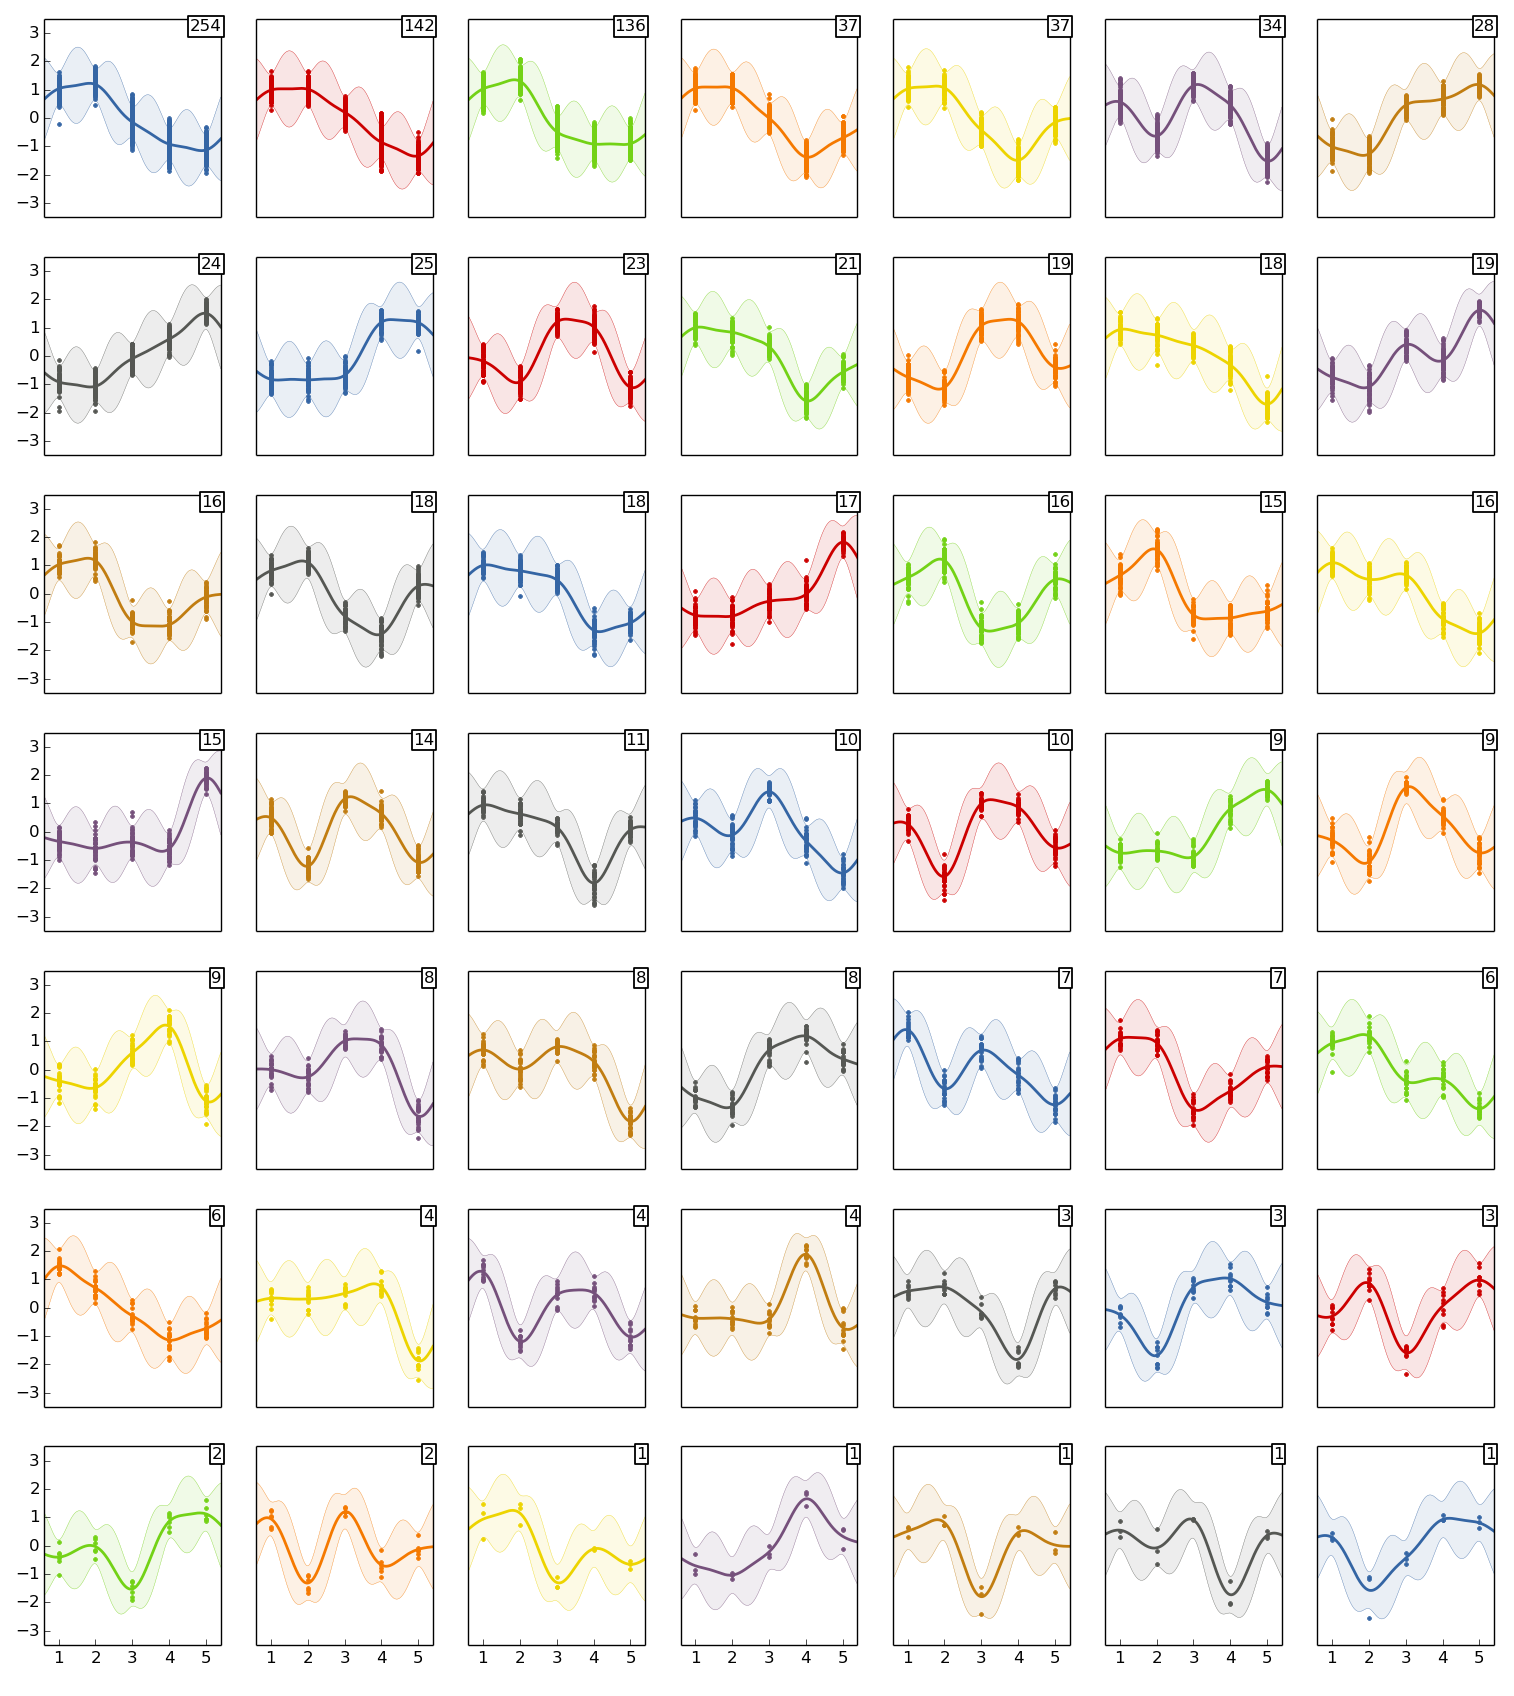
\includegraphics[width=\textwidth,keepaspectratio]{clsCElegans11genes_2.png}
		\rule{35em}{0.5pt}
	\caption[Clustering Gene Expression dataof \textit{C.elegans}]
		{Clustering Gene Expression data of \textit{C.elegans}} % TODO
	\label{fig:clsCelegans}
\end{figure}


\subsection{Kernel Design with Coregionalization}\label{subSec:Kernel_Design_with_Coregionalization}
Gaussian process models have been used already to capture structure in the data arising from temporal correlation. Our innovation is to realise that there is actually additional correlation structure relating to the genetic background of the organism (in our case, the mice strains) and the status as control/experiment (in our case the presence or absence of the SOD1 mutation). By acknowledging such structure in the covariance matrix we can increase the power of our method. Standard approaches force each of these conditions to be fully independent. Our model allows the correlation structure to be learned.
\begin{figure}
 \begin{center}
  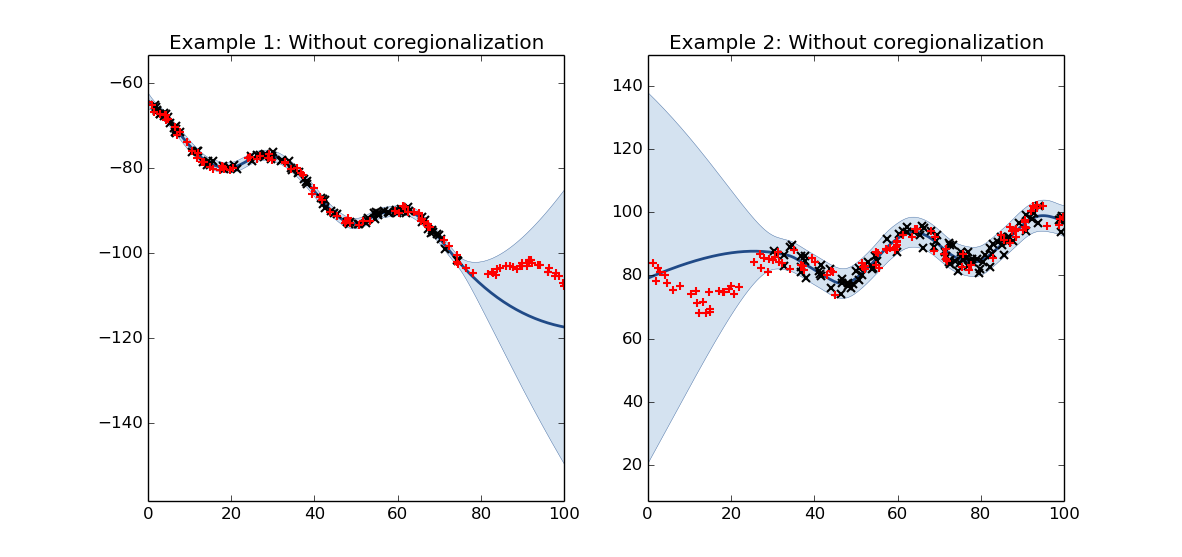
\includegraphics[width=\textwidth]{coreExample_No.png}
  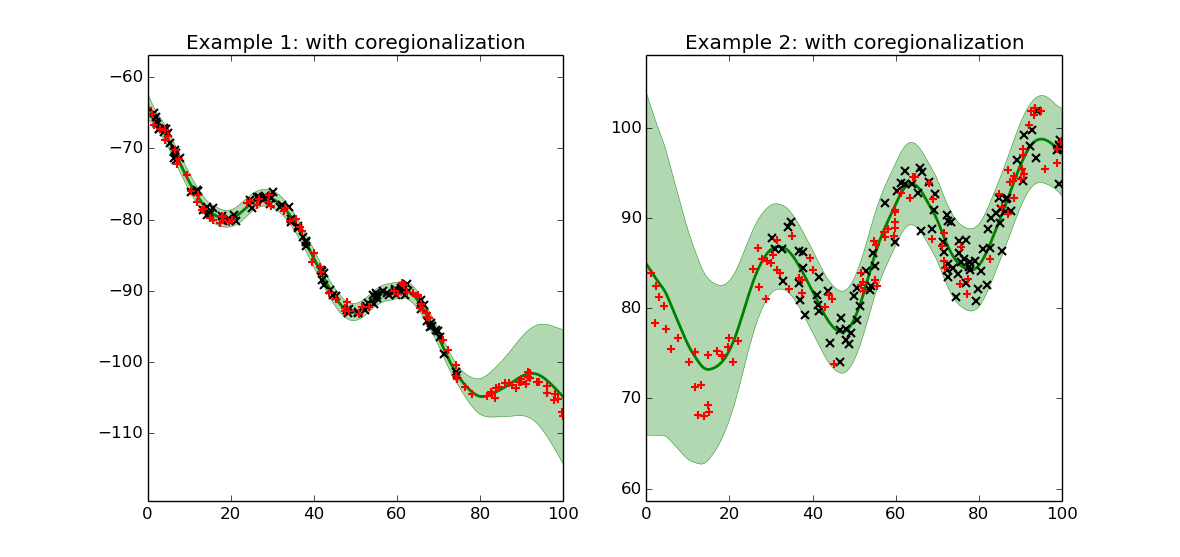
\includegraphics[width=\textwidth]{coreExample_with.png}
    \caption [Simple demonstration of  \emph{coregionalization} model] 
    {Simple demonstration of regression using \emph{coregionalization} model with Gaussian process. Here, training data marked with black, while red represents test data. Solid line represents a posterior mean function and shaded area represents 95\% confidence interval. The independent models (top-left and top-right) do not share information across outputs. The independent models tend to return to the prior assumptions in the regions where there is no training data specific to an output. While the coregionalized model (bottom-left and bottom right) shares information across outputs. Here both outputs have associated patterns, where there is no training data the fit is better with the coregionalized model. A Jupyter Notebook demo of coregionalization using Gaussian processes is available at the GPy \cite{gpy2014}.
  \label{fig:demoCoregionalization}}
 \end{center}
\end{figure}

Our formalism for introducing correlations across conditions and strains is the \emph{coregionalization} principle (\cite{Alvarez:2011}) that originates in geostatistics (\cite{Wackernagel:2003}). \emph{Coregionalization} matrices allow us to share the information between genetic background and replicates. In machine learning language this approach is sometimes known as \lq multi-task learning \rq (\cite{Bonilla:2007}) where each condition and strain is assumed to be a different task. However, in statistical terms it is simply a multi-variate regression or a multiple output model.

An appropriate general model that can capture the dependencies between all the data points and conditions is known as the linear model of coregionalization (LMC) is a model where output is a linear combination of independent random functions. (A detail explanation of the \emph{coregionalization} model is available at \cite{Alvarez:2011, Alvarez:2012}). If we can consider our problem with a set of $D$ output functions for $\textbf{x}\epsilon\mathbb{R}^p$ input domain, then output function $\{ f_d\left(\textbf{x}\right)\}^D_{d=1}$ of $LMC$ can be expressed as
\begin{equation} \label{eq:LMC}
f_d\left(\textbf{x}\right)=\sum\limits_{q=1}^Q a_{d,q}u_q\left(\textbf{x}\right)
\end{equation}

Here the interpretation is that $\{u_q^i\left(\textbf{x}\right)\}^{R_q}_{i=1}, i= 1,..., R_q$ are a set of functions that each share the same covariance function (one can think of them as some form of underlying \emph{latent} processes that determine system behaviour). The parameters $a_{d, q}$ represent the relationship between a given latent function, $q$ and an observed condition and or strain. If we consider there can be several different covariance functions associated with separate latent sets then equation \ref{eq:LMC} is expressed as
\begin{equation} \label{eq:LMClatent}
f_d\left(\textbf{x}\right)=\sum\limits_{q=1}^Q \sum\limits_{i=1}^{R_q} a^i_{d,q}u^i_q\left(\textbf{x}\right)
\end{equation}
and the cross covariance function between $f_d\left(\textbf{x}\right)$ and 
$f_{d\textprime}\left(\textbf{x}\right)$ in terms of the function $u^i_q\left(\textbf{x}\right)$
is given by
\begin{equation} \label{eq:LMCcov}
\begin{split}
&\text{cov} \left[ f_d\left(\textbf{x}\right), f_{d\textprime}\left(\textbf{x\textprime}\right)\right]=\\
&\sum\limits_{q=1}^Q \sum\limits_{q\textprime=1}^Q \sum\limits_{i=1}^{R_q} \sum\limits_{i\textprime=1}^{R_q}
a^i_{d,q}a^{i\textprime}_{d\textprime,q\textprime} 
\text{cov} \left[ u^i_q\left(\textbf{x}\right),u^{i\textprime}_{q\textprime}\left(\textbf{x\textprime}\right) \right].
\end{split}
\end{equation}

\begin{figure}
 \begin{center}
  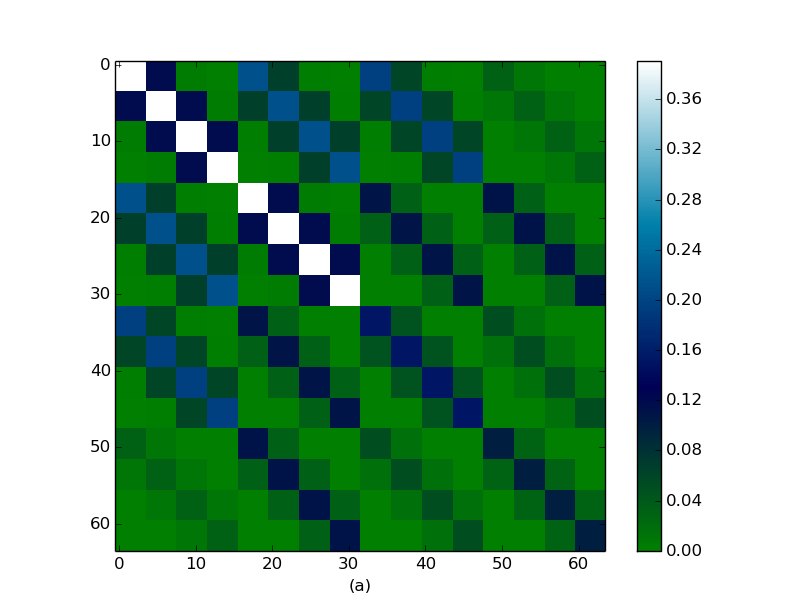
\includegraphics[width=.49\textwidth]{fXkern.png}
  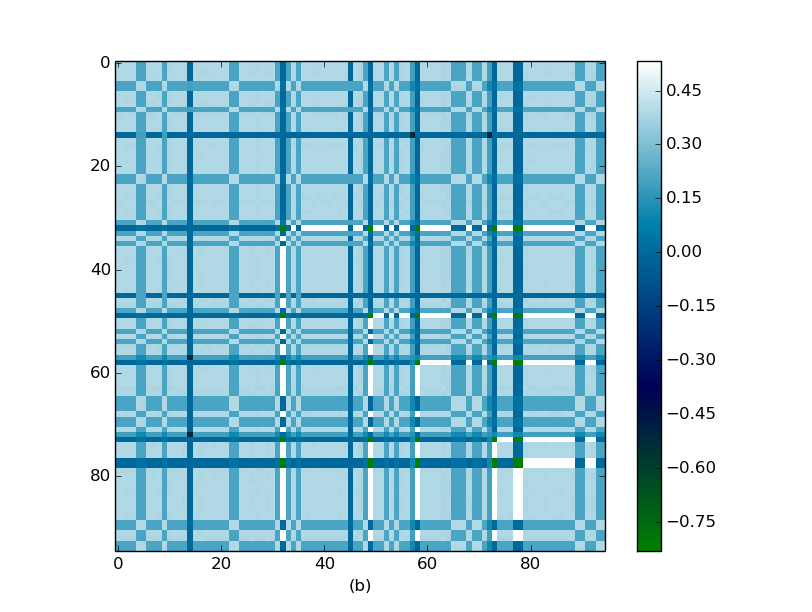
\includegraphics[width=.49\textwidth]{fYkern.png}
  \caption {Simple representation of kernels- (a). \emph{Coregionalization} kernel in the input space  with $64\times64$ dimensions; (4 strains ($129Sv-SOD1, 129Sv-Ntg, C57-Ntg$ and $C57-SOD1$) $\times$ 4 replicates $\times$ 4 time points or stages of the disease). With a closer look, we can find four primary segments, where every quarter can be treated as a strain; Each quarter has four more segments which indicate four replicates; Each replicate has a further four segments which represent four different disease stage or time points (b). kernel after optimization considering top most 100 (an arbitrary suitable number for visualization) differentially expressed genes. This is a realization of covariance between genes, where every pixel is computed using the \emph{coregionalization} kernel.
  \label{fig:kernel}}
 \end{center}
\end{figure}

For the so-called homotopic case (\cite{Alvarez:2011, Wackernagel:2003}) the covariance matrix for the joint process $\textbf{f}$ can be rewritten as a sum of Kronecker products, finally we can write the covariance as
\begin{equation} \label{eq:LMCcovK}
\textbf{K}_{f,f}=\sum\limits_{q=1}^Q \textbf{A}_q\textbf{A}^{\top}_q \otimes \textbf{K}_q
=\sum\limits_{q=1}^Q \textbf{B}_q \otimes \textbf{K}_q
\end{equation}
where $\otimes$ represents Kronecker product, $\textbf{A}_q \epsilon \mathbb{R}^{D\times R_q}$ and $\textbf{B}_q$ is the \emph{coregionalization} matrix\footnote{In Chapter \ref{ch:GP_Model_of_TFAs} Section \ref{sec:Model_for_TFA} we developed a model for transcription factor activity and used intrinsic coregionalization model. There the matrix $\boldsymbol{\Sigma}$ was termed as the coregionalization matrix. Coregionalization matrix $\boldsymbol{\Sigma}$ of \ref{eq:K_intrinsic_coregionalization} and coregionalization matrix $\textbf{B}_q$ of Equation \ref{eq:LMCcovK} have the similar realization.}. The positive semi-definite covariance functions of the latent processes, $k_q\left(\textbf{x},\textbf{x}\textprime\right)$ can be chosen from wide range of covariance functions. 

Figure \ref{fig:demoCoregionalization} shows a simple demonstration of regression using coregionalization model with Gaussian process. Here, the independent models do not share information across outputs and tend to return to the prior assumptions in the regions where there is no training data specific to an output. While the coregionalized model shares information across outputs. Here both outputs have associated patterns, where there is no training data the fit is better with the coregionalized model. We introduced coregionalization while developing the kenels in the hierarchical Gaussian process clustering. So, the information between the conditions, replicates and disease stages will be shared. 

In our clustering problem we used a combination of exponentiated quadratic kernel (also known as squared exponential or RBF kernel) to describe the properties of the function which underlay each cluster. We used a white noise kernel in additive form to deal with the noise of the process. The experimental conditions of acquisition of gene expression measurements cannot be ideally controlled, so the measurements could be corrupted by noise, incorporated either at the biological origin or introduced in the measurement process. Figure \ref{fig:kernel} shows the representation of the coregionalized kernel in the input space and the representation of an optimized kernel where we considered only 100 (top most differentially expressed; an arbitrary number suitable for visualization) genes.

\subsection{Clustering}
Our aim was to discover groups of genes that were exhibiting the same functional behaviour across times and conditions. Our coregionalization approach allows us to cluster these similar functional behavioural genes through a mixture of Gaussian process models: each component is a function over time, genetic background and condition.

%% Clustering gene expression time series is aimed at discovering a group of associated or co-regulated
%% genes. It is assumed that they share an underlying time series and are potentially involved in some specific 
%% biological process.
Partitioning genes into clusters are done by inference. Using Dirichlet process prior for mixing coefficients and partitioning \cite{Dunson:2010} proposed a method where Gaussian process was used to model the function within a cluster. This mechanisms leads to Gibbs sampling. In this process, at every Gibbs step a gene is removed from the cluster and then reallocated it stochastically. The whole process can be slow in practice. A potentially improved model was proposed by \cite{Hensman:2013}, where they consider the structure of covariance across the gene and separately across replicates. They used a variational lower bound for model inference. Each gene is placed in an individual cluster and later merged with a greedy selection process to maximize the log marginal likelihood of time series data. Hyperparameters are optimized when no merges are possible to improve the overall marginal likelihood. Then an expectation maximization algorithm is used with the new covariance function\footnote{The idea is implemented in a tool named named \emph{GPClust}, available at \url{https://github.com/jameshensman/GPclust}} (\cite{Hensman:2013}).

\section{Dataset and Results}

\paragraph{Microarray Data Analysis:}
We used the Affymetrix data from \cite{Nardo:2013}.  In this experiment spinal cord tissues were obtained from $C57$ and $129Sv$ transgenic $SOD1^{G93A}$ mice and age-matched non-transgenic littermates at the presymptomatic, the early symptomatic (onset) stage, symptomatic and end stage.  The transcription profiles of laser captured motor neurons isolated from the lumbar ventral spinal cords of the rapid progressor $(129Sv-SOD1^{G93A})$, slow progressor $(C57-SOD1^{G93A})$ mice at four stages of the disease (presymptomatic, onset, symptomatic, end stage) and respective non-transgenic littermates were generated using the murine GeneChip Mouse Genome 430 2.0 Plus (Affy MOE4302). We used \emph{Bioconductor}\footnote{Bioconductor is an open-source computational framework for the analysis of high throughput genomic data in the R programming language.} pacakge \emph{Puma} (\cite{puma}) to extract the point estimates of gene expression levels from the GeneChip Affymetrix data.

\begin{figure}
	\centering
		%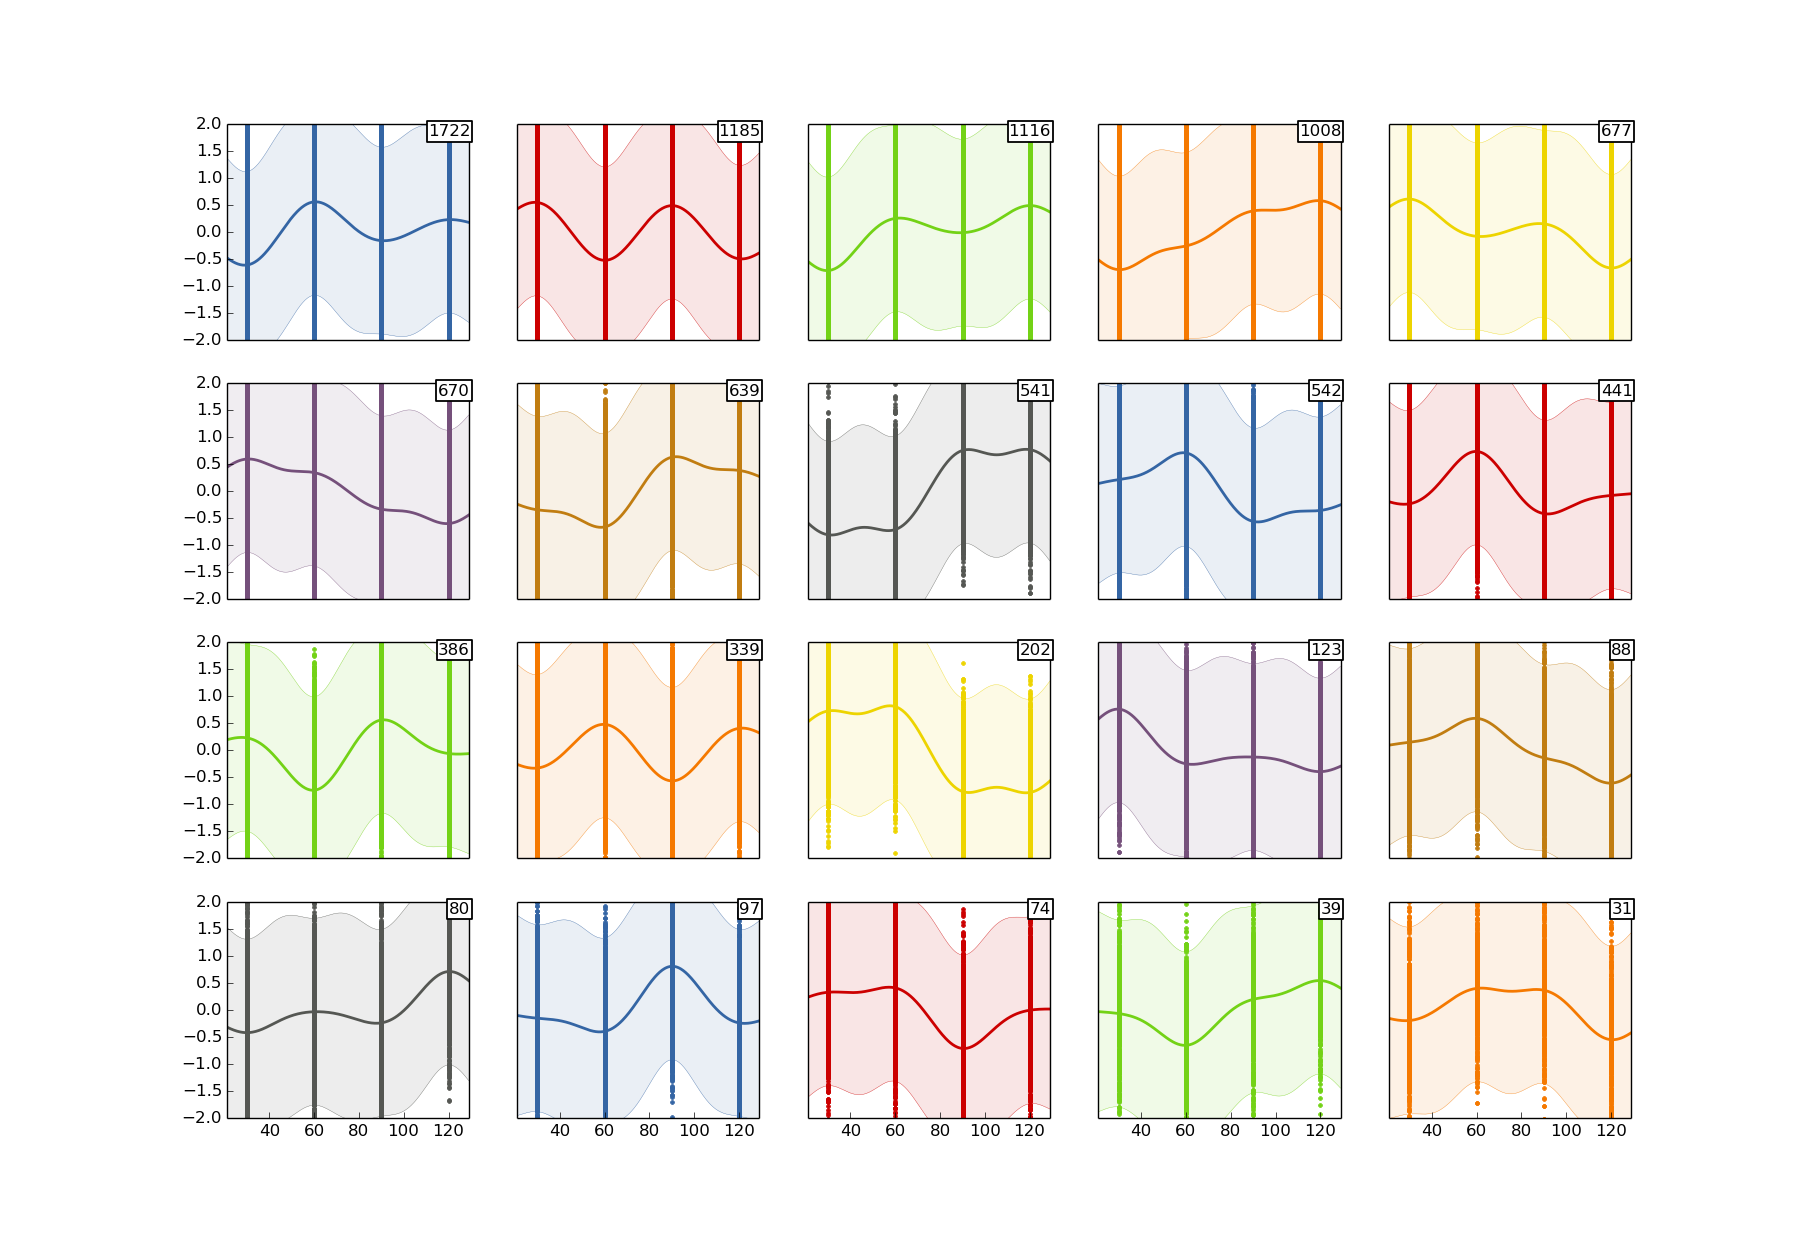
\includegraphics[width=\textwidth,keepaspectratio]{clsALSnoCore10000g.png}
		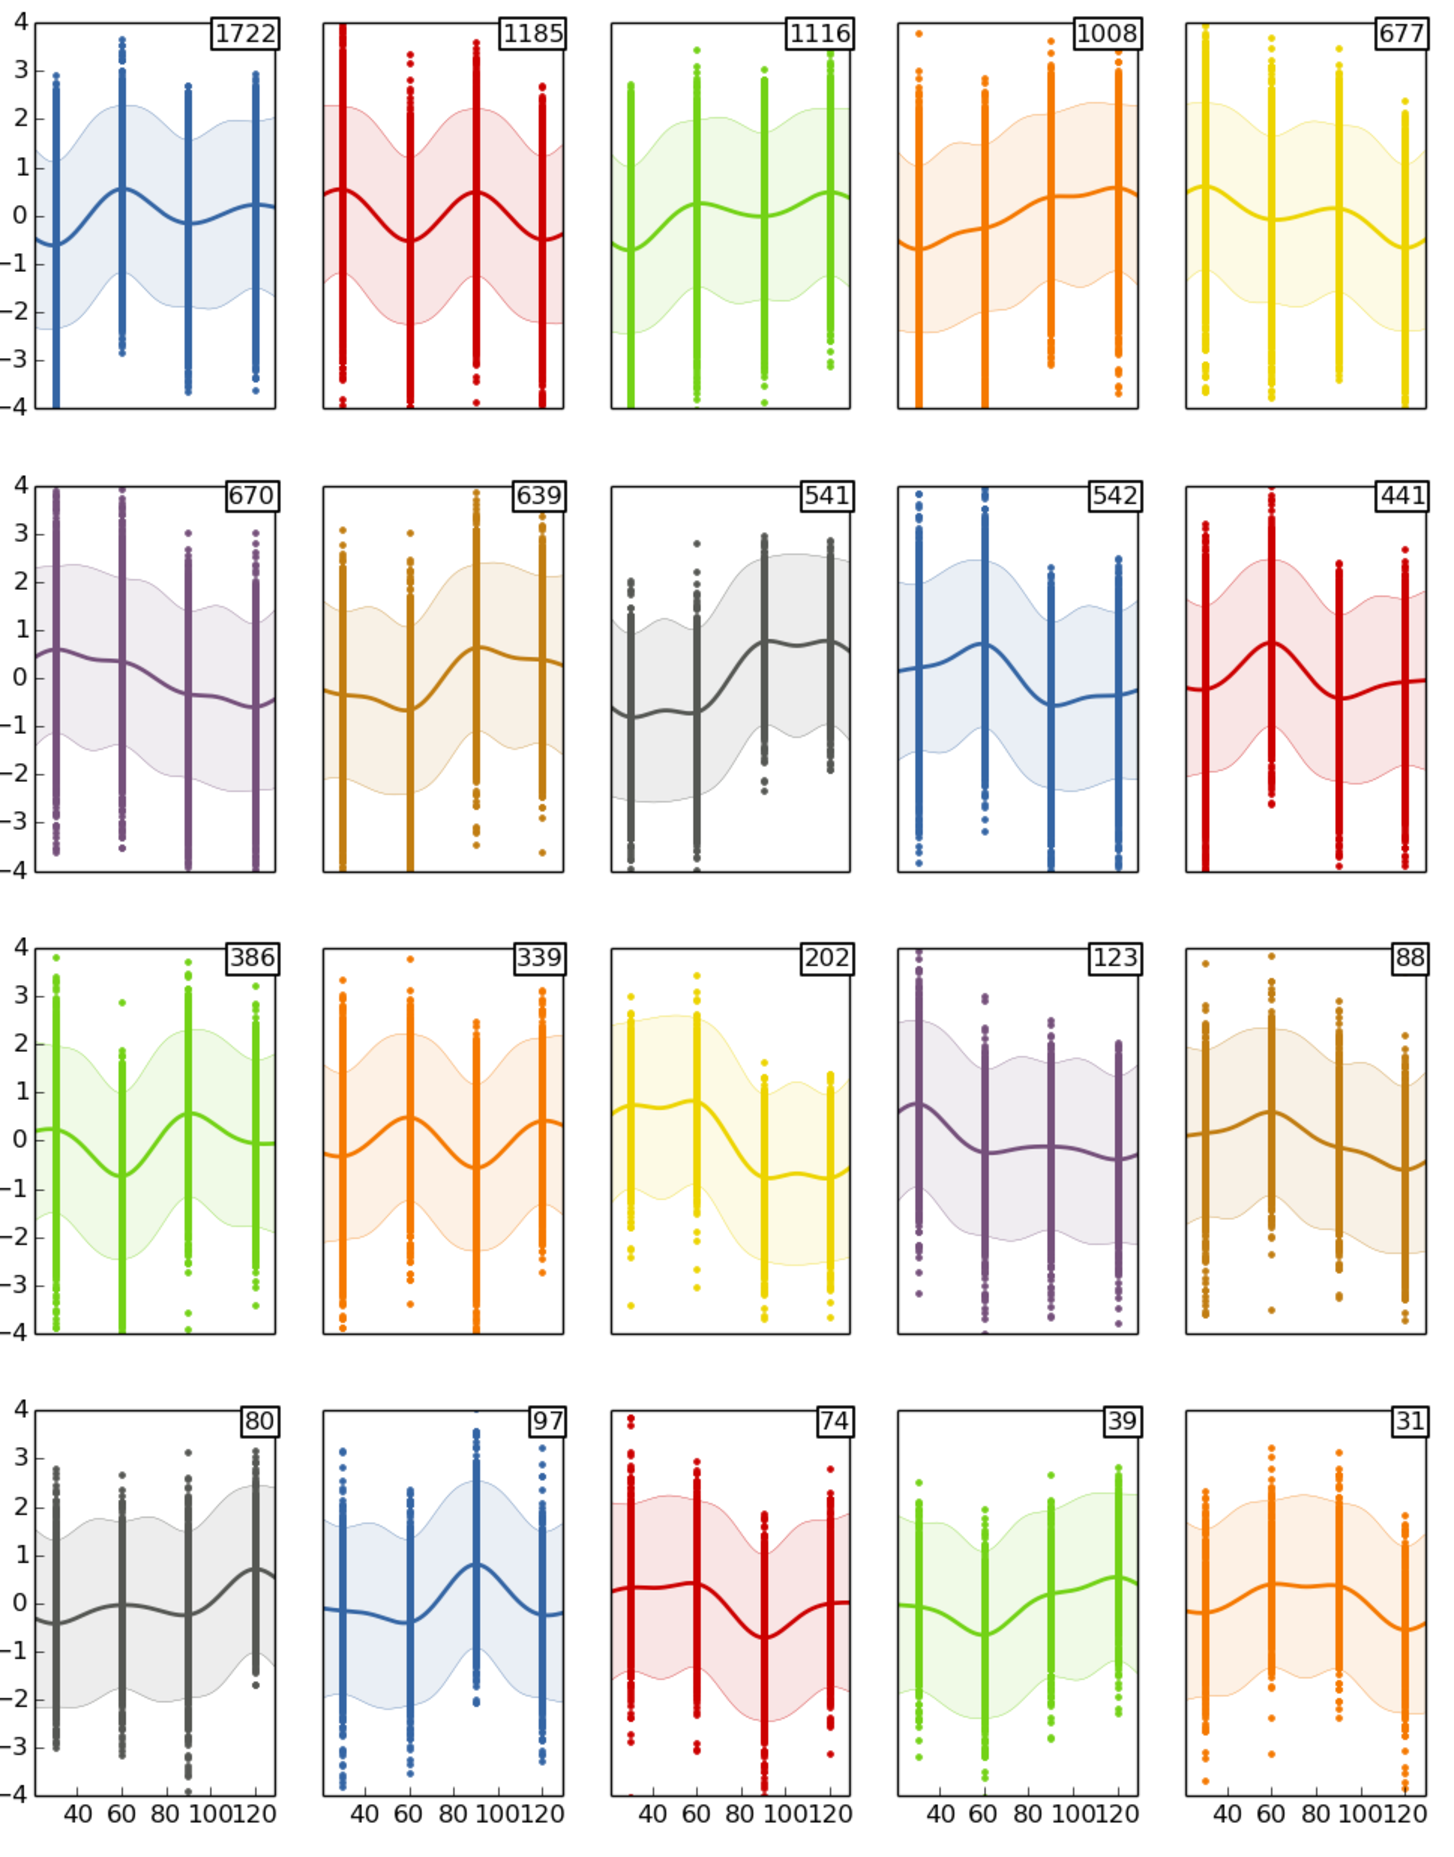
\includegraphics[width=\textwidth,keepaspectratio]{figure_noCore.pdf}
		\rule{35em}{0.5pt}
	\caption[Clustering gene expression data no coregionalization]
		{Clustering gene expression data using the method proposed by \cite{Hensman:2013}. Along $x$-axis the four time stages are pre-symptom, onset, symptom and end-stage (all the data points together formed like solid vertical lines). Number at the corner indicates number of genes belong to this cluster. Solid line represents a posterior mean and shaded area represents 95\% confidence interval. We used top most 10,000 differentially expressed genes and they were clustered among 20 clusters. The number of the clusters and the genes belongs to a specific cluster was selected by the algorithm.}
	\label{fig:clsNoCoregionalization}
\end{figure}

\begin{figure}
 \begin{center}
    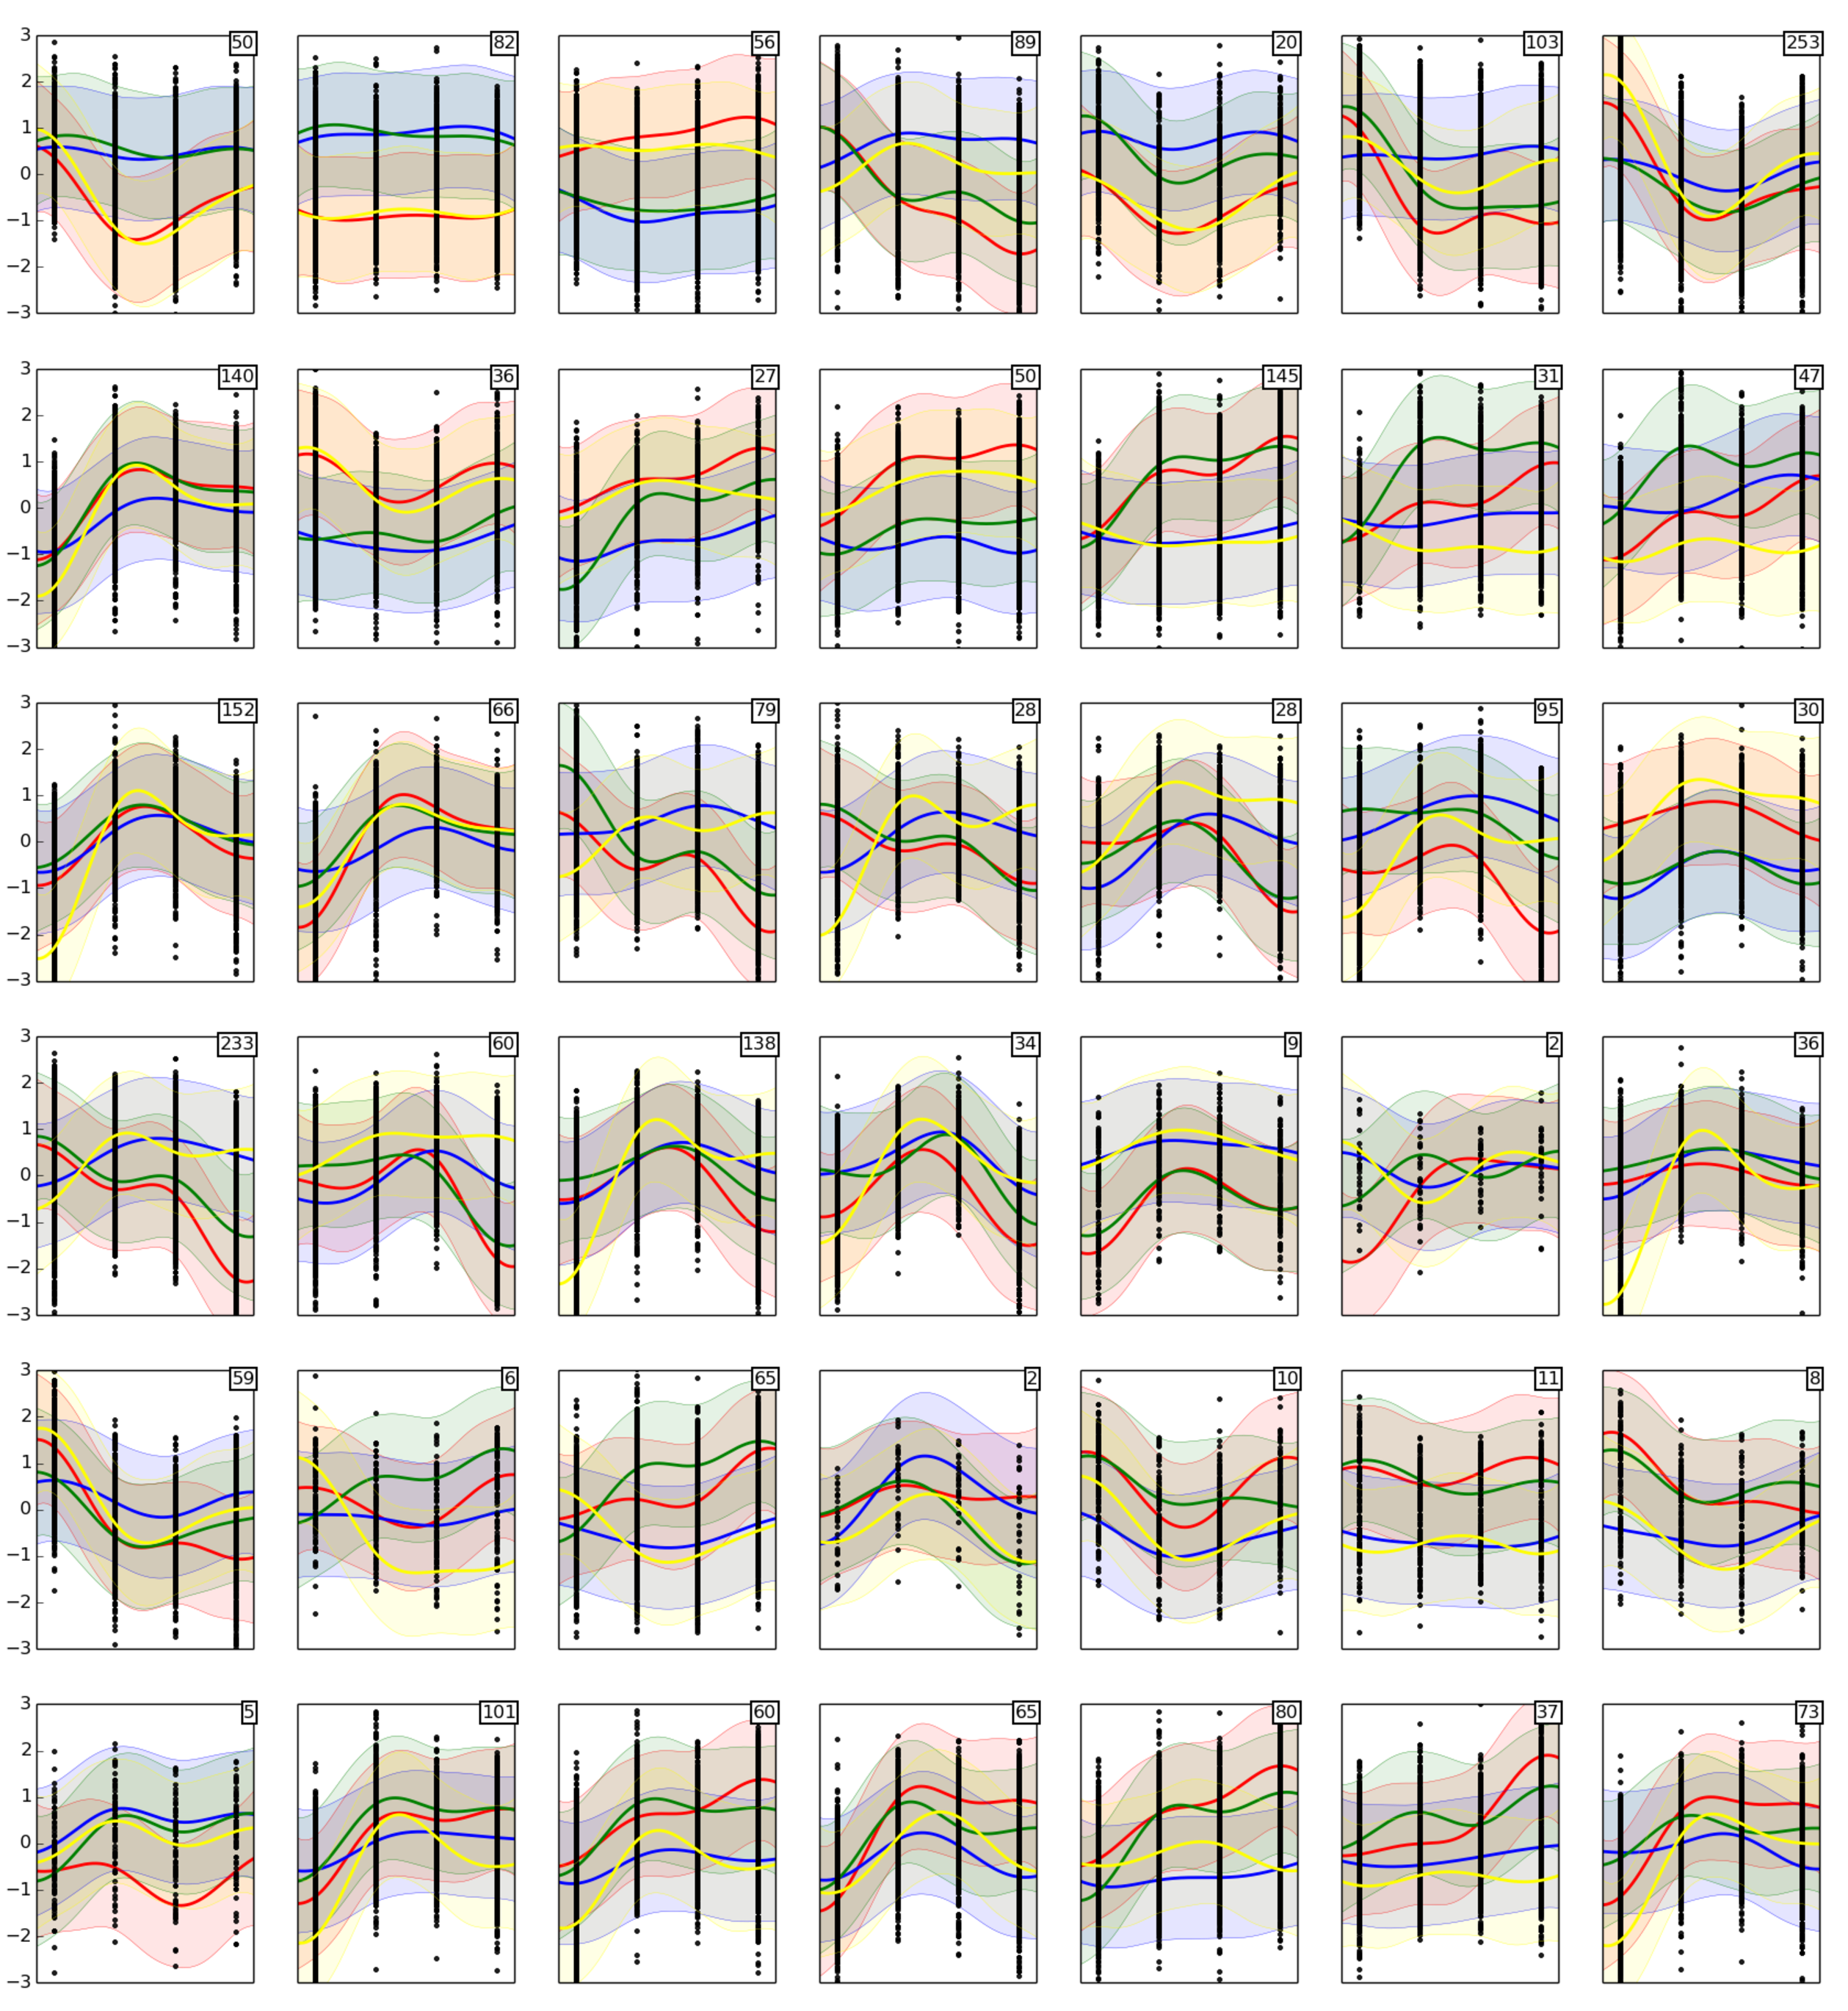
\includegraphics[width=\textwidth]{fig52.pdf}
    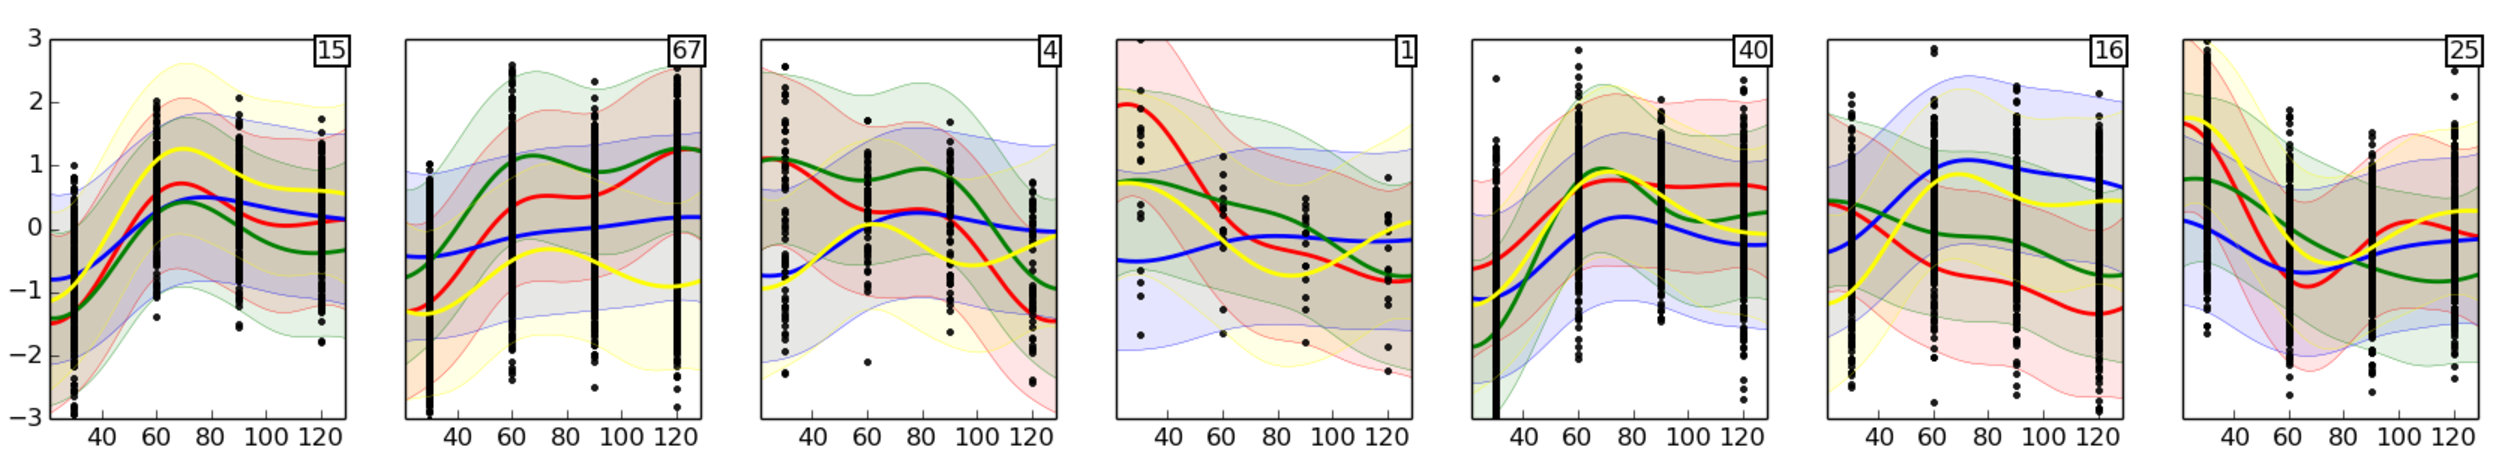
\includegraphics[width=\textwidth]{fig522.pdf}
    %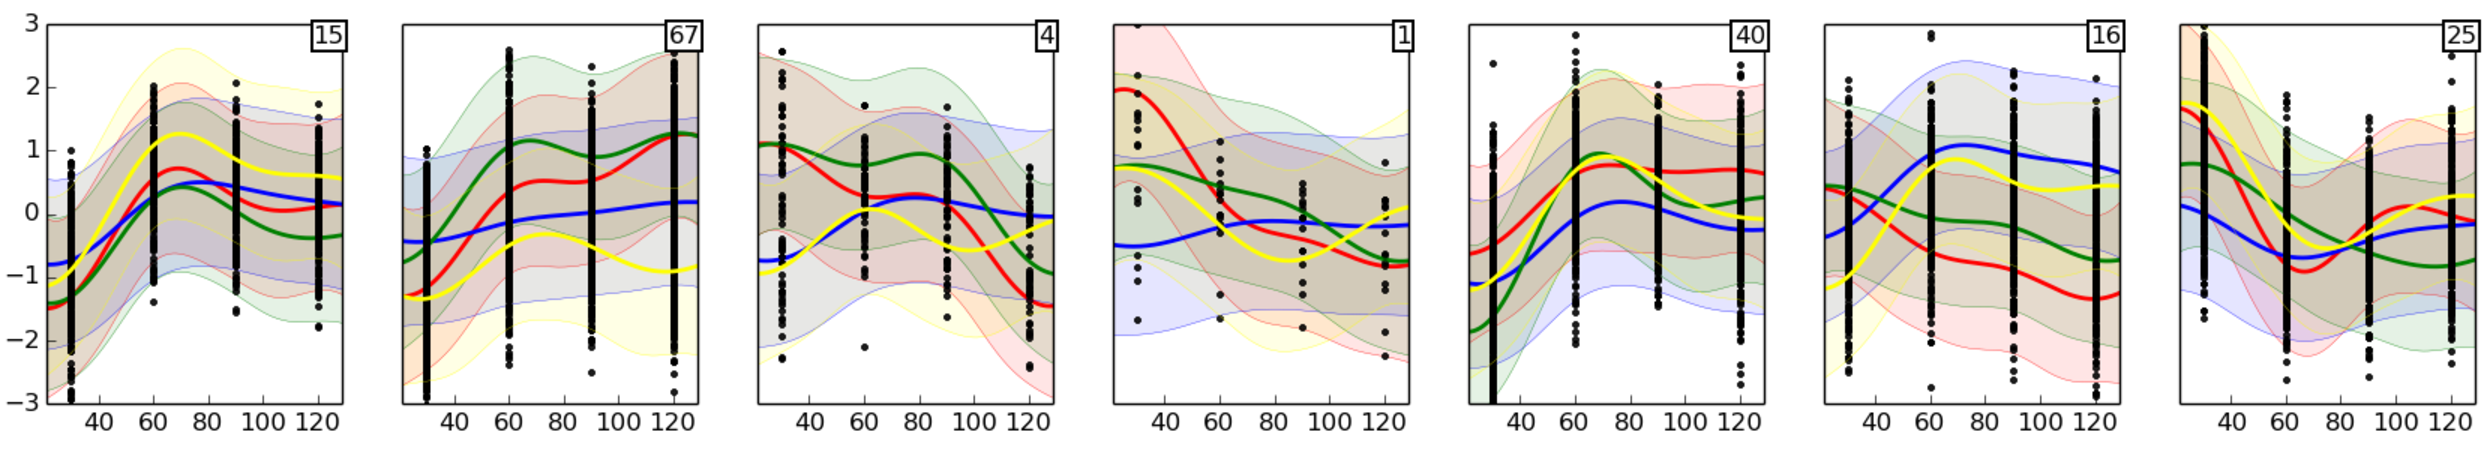
\includegraphics[width=\textwidth]{fig523.pdf}
    %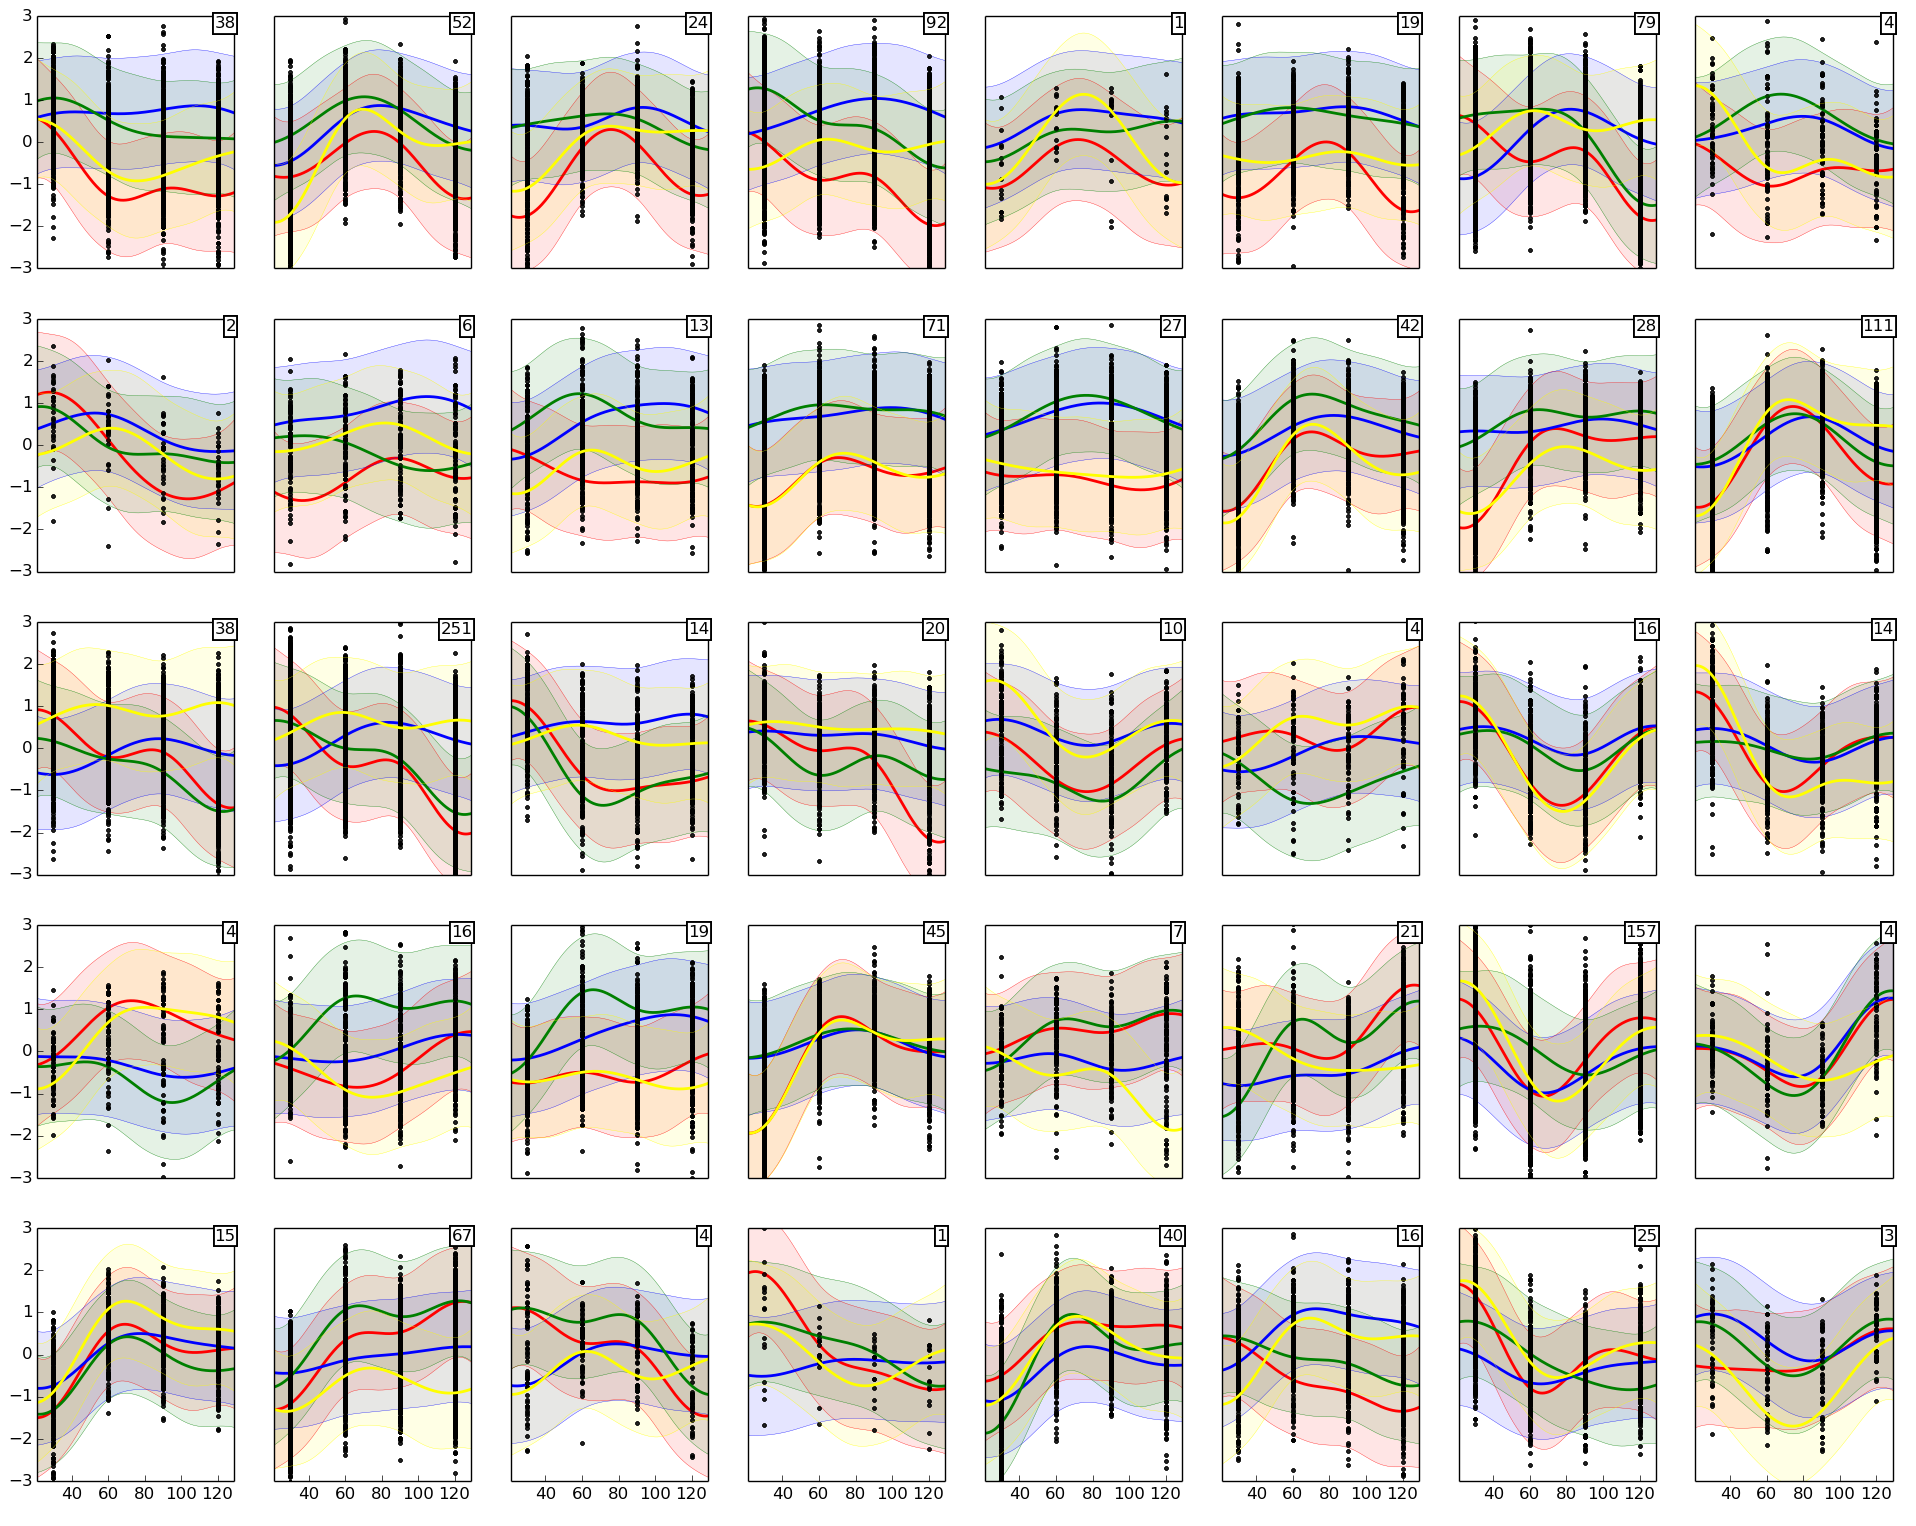
\includegraphics[width=\textwidth]{new40Cluster.png}
    \caption [Clustering genes expressions using hierarchy of Gaussian processes] 
    {Clustering genes expressions using hierarchy of Gaussian processes. Some representative clusters from the 203 clusters generated (top to bottom, left to right: cluster 1 to 7, 16 to 22, 31 to 37, 46 to 52, 61 to 67, 76 to 82 and 196 to 202). Along $x$-axis the four time stages are pre-symptom, onset, symptom and end-stage (all the data points together formed like solid vertical lines). Four different colours yellow, red, green and blue are representing four mouse strains $129Sv-SOD1, 129Sv-Ntg, C57-Ntg$ and $C57-SOD1$ respectively. Number at the corner indicates number of genes belong to this cluster. Solid line represents a posterior mean function and shaded area represents 95\% confidence interval.\label{fig:fewClusters}}
 \end{center}
\end{figure}

\begin{figure}
 \begin{center}
 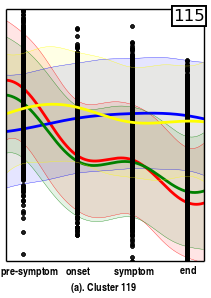
\includegraphics[width=.23\textwidth]{newCluster119.png}
 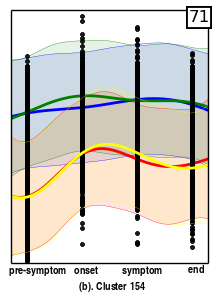
\includegraphics[width=.23\textwidth]{newCluster154.png}
 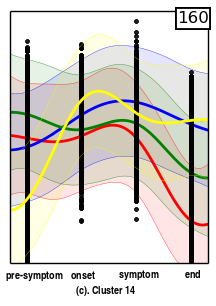
\includegraphics[width=.23\textwidth]{newCluster14.png}
 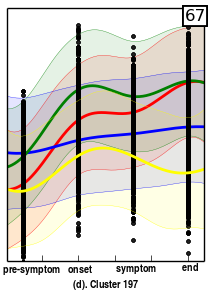
\includegraphics[width=.23\textwidth]{newCluster197.png}
  \caption [Few examples of clusters with different dynamics]
  {Along $x$-axis of each individual figure four time stages are pre-symptom, onset, symptom and end-stage. Four different colours yellow, red, green and blue are representing four mouse strains $129Sv-SOD1, 129Sv-Ntg, C57-Ntg$ and $C57-SOD1$ respectively. Examples of clusters where genes from different phenotypic background have different behaviour in time series expression. We used a simple numbering system to represent our clusters and here we are presenting (Figure left to  right) cluster119, cluster154, cluster14 and cluster197. Cluster119 showing the clear separation between transgenic group ($129Sv-SOD1$ and $C57-SOD1$) with non-transgenic mouse model($129Sv-Ntg$ and $C57-Ntg$), while cluster154 separating mouse $C57$ from mouse $129sv$. Cluster14 and cluster197 showing the different characteristics of $129Sv-SOD1$ from other three models where it is increasing sharply or becoming very low respectively after the end stage. \label{fig:fourSampleClusters}}
 \end{center}
\end{figure}


\paragraph{Select differentially expressed genes:}
All the gene expression time series data extracted from Affymetrix data might not be differentially expressed and filtering out the requisite genes is obvious. Considering the temporal nature of data \cite{Kalaitzis:2011} analysed time series gene expressions and filter the quiet or inactive genes from the differentially expressed ones using Gaussian process.  In addition identifying genes that have a good signal-to-noise ratio (SNR) is also used to filter down the total number of genes that need further analysis. We can rank the genes by the ratio of the mean replicate-wise variance to the variance of the replicate-wise means. In our analysis we used a combination of both approaches.  First we made the initial ranking of the gene expressions (45,037 genes for our case) using method of \cite{Kalaitzis:2011} and then we use the SNR to choose 10,000 genes \footnote{10,000 is an arbitrary choice. We did the similar experiments choosing 2,000, 5,000 and 15,000 genes and found similarity in the results with minor variations.} for further analysis. The gene expression levels of each replicates were normalized to zero-mean over all the samples before the filtering.

\paragraph{Cluster analysis:} 
In the previous selection stage we choose 10,000 genes from the total of 45,037 probe sets which were more dynamically differentially expressed. We applied our own hierarchical Gaussian process cluster model on these genes and collected the results for further experiments. Figure \ref{fig:fewClusters} shows a small part of our result. For any individual graph, along $x$-axis the four time stages are pre-symptom, onset, symptom and end-stage. We have used four different colours (yellow, red, green and blue) to separate four mouse strains ($129Sv-SOD1, 129Sv-Ntg, C57-Ntg$ and $C57-SOD1$ respectively). Any individual cluster contains a number of genes which might be biologically associated or co-regulated and we mention the number of the genes belong to that cluster at the corner of the plot. In the plot a solid line represents posterior mean function and shaded area represents 95\% confidence interval. We have found a total of 203 different clusters with a variation of number of genes for any individual cluster. All the clusters were indicating different dynamic behaviour of the gene set. We found a number of clusters were attractive for further analysis but the detail analysis of every cluster is beyond the scope of this study. We included some examples in the Figure \ref{fig:fourSampleClusters}. We have limited our consideration to the clusters where the strain $129Sv-SOD1$ (yellow color in our representation) has different characteristics and focussed our consideration for further analysis.
\begin{figure}
	\centering
		%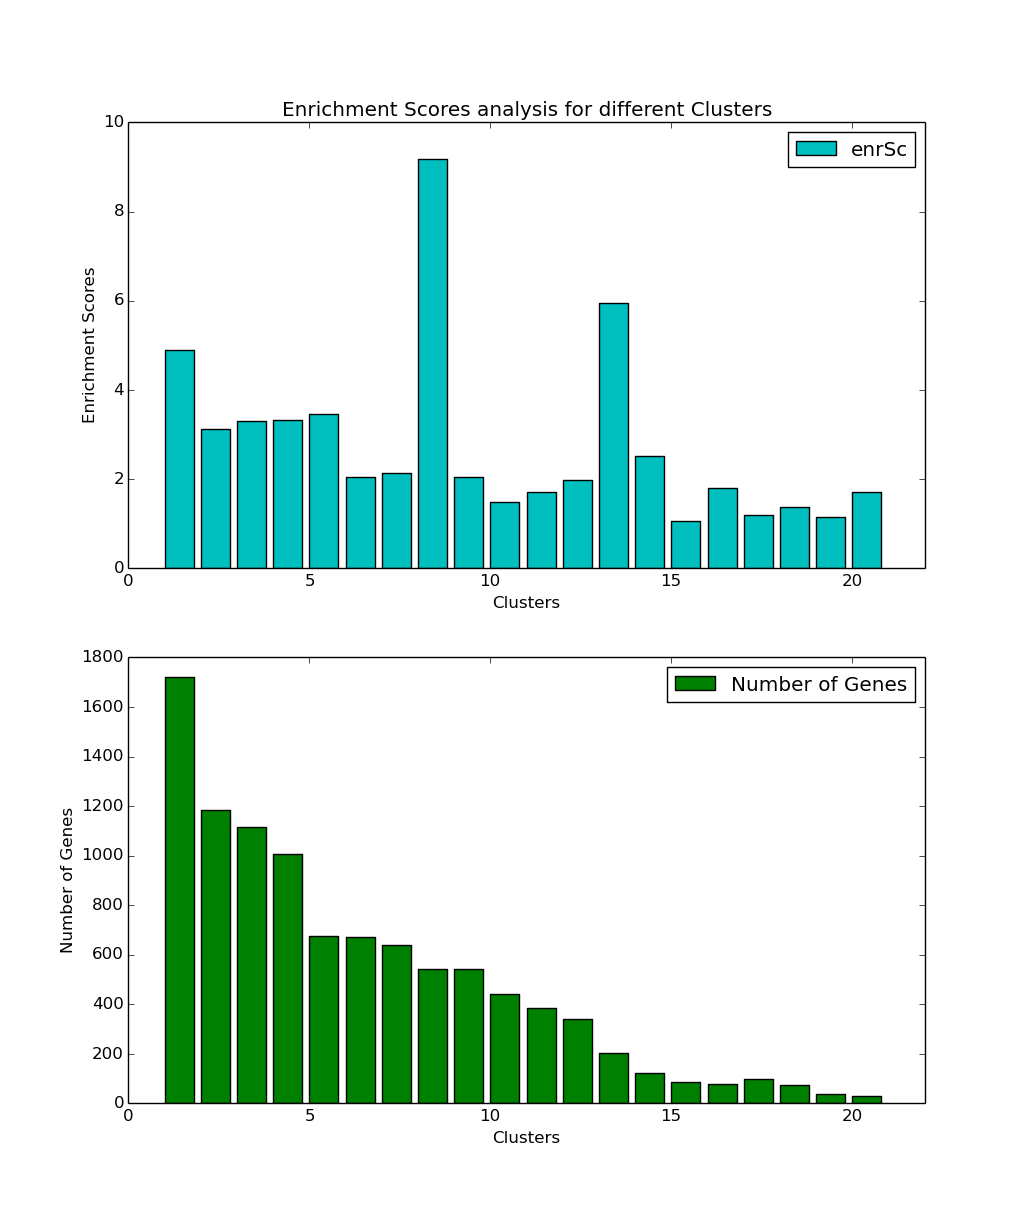
\includegraphics[width=0.7\textwidth,keepaspectratio]{barGraphNoCore10000g.png}
		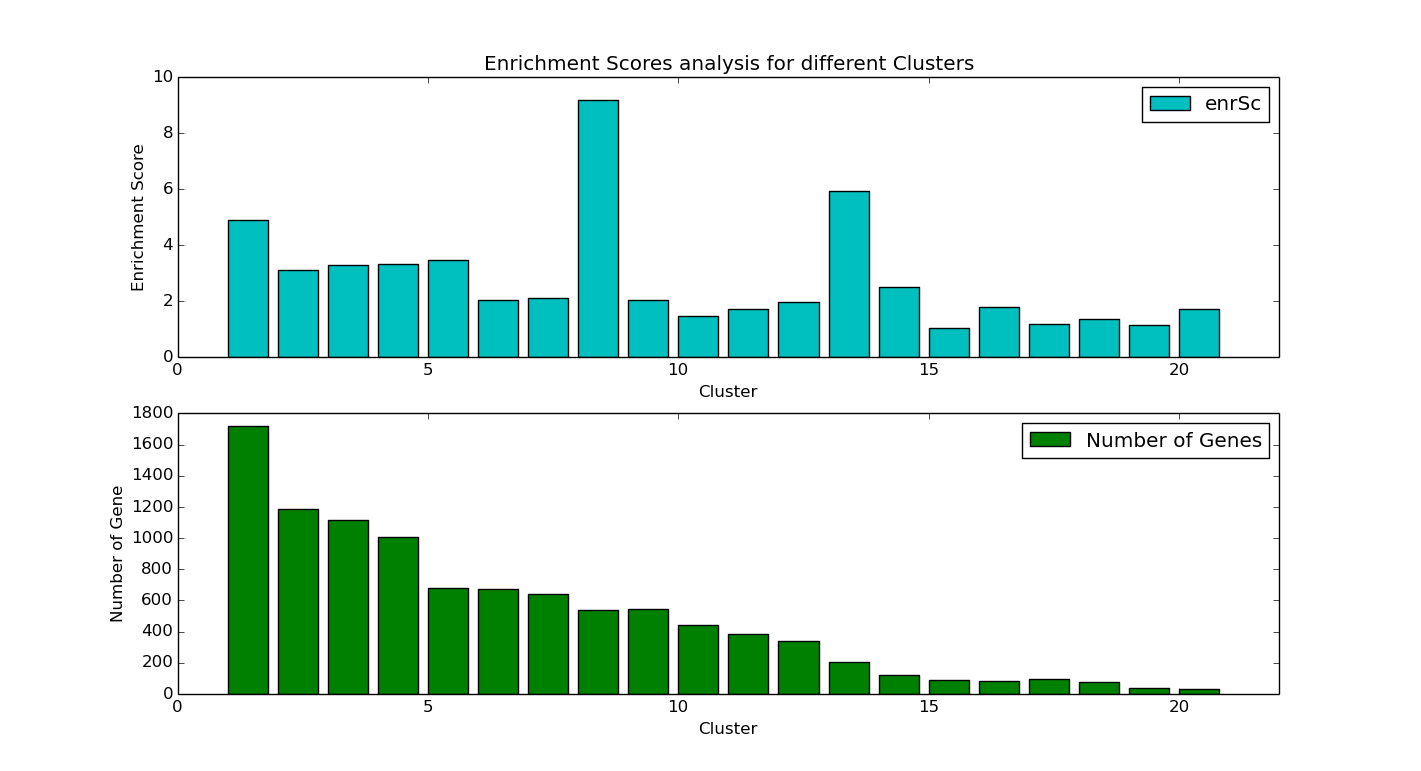
\includegraphics[width=0.9\textwidth,keepaspectratio]{enrichnoCore.png}
		\rule{35em}{0.5pt}
	\caption[Enrichment scores analysis for different clusters without \emph{coregionalization}]
		{Enrichment scores analysis without \emph{coregionalization}. Figure at the top shows the enrichment score for different clusters, where $x$-axis is the cluster number and $y$-axis shows the  enrichment score of that cluster. Figure at the bottom shows the number of genes belongs to any specific cluster.}
	\label{fig:enrichNoCoregionalization}
\end{figure}

\paragraph{Enrichment score analysis:}
\begin{figure}
 \begin{center}
 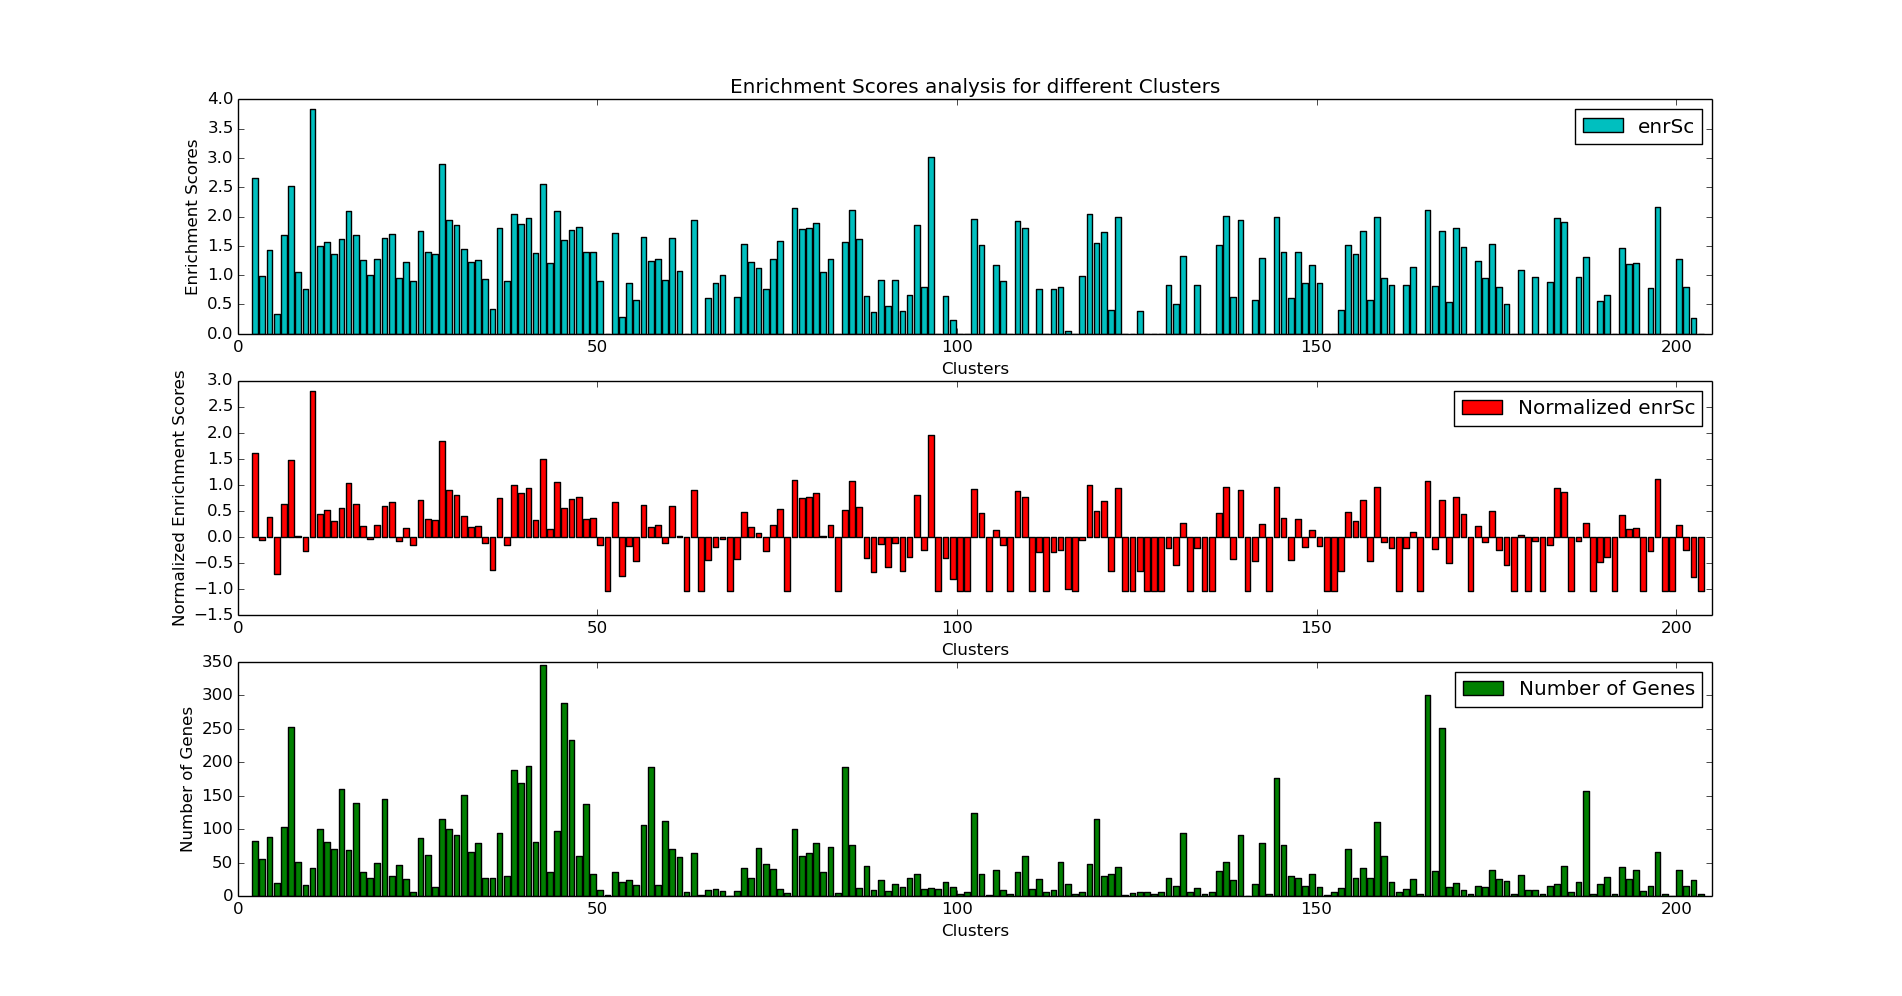
\includegraphics[width=\textwidth]{EnrichmentScoresGenes.png}
  \caption [Enrichment scores analysis for different clusters] 
  {Enrichment scores analysis. Figure at the top shows the enrichment score for different clusters where $x$-axis is the cluster number and $y$-axis shows the enrichment score of that cluster. Figure located at the middle shows the normalized score (mean enrichment score is 1.05). While the bottom figure shows the number of genes belongs to any specific cluster.
  \label{fig:EnrichmentScores}}
 \end{center}
\end{figure}

A typical biological process is regulated with a group of genes. If we apply a high throughput screen technology then the co-functioning genes are more likely to appear together with a higher potential (or enrichment) score. These logical reasons instigate the analysis of a gene list or group of genes moving from individual gene oriented view. The enrichment score is a quantitative measure derived from some well known statistical methods like Binomial probability, hyper-geometric distribution, Chi-square, Fisher's exact test. In a previous study, \cite{Huang:2009Enrichment} reported about 68 Bioinformatics tools to compute the enrichment score and grouped them in three major categories. \emph{DAVID} \cite{Huang:2009David} is a widely used tool developed based on Fisher's exact and extensively used for singular enrichment analysis (SEA) and modular enrichment analysis (MEA). We used DAVID on our clusters of genes to calculate the enrichment score for individual clusters.  Figure \ref{fig:enrichNoCoregionalization} and Figure \ref{fig:EnrichmentScores} shows the result the results of enrichment score analysis. In a functional annotation clustering example \cite{Huang:2007} analysed a group of genes and used enrichment score of 1.3 as a threshold value to decide whether a list of genes are enriched or not. Here for our 203 clusters the mean enrichment score is 1.05 and we have found at least 15 clusters have an enrichment score of $\geq 2$. We choose these top 15 annotation clusters out of total 203 clusters for further analysis.

\begin{table}
    \begin{tabularx}{1.0\textwidth}{ l X l l l }
      \toprule
	\textbf{Annotation Cluster 1}	& \textbf{Enrichment Score: 2.16}	& \textbf{Count}	& \textbf{P\_Value}	& \textbf{Benjamini}\\ %Benjamini
      \midrule
	GOTERM\_CC\_FAT	& organelle inner membrane		& 9	& 3.0E-5	& 4.5E-3\\ 
	GOTERM\_CC\_FAT	& mitochondrial inner membrane		& 8	& 1.6E-4	& 1.2E-2\\ 
	GOTERM\_CC\_FAT	& organelle membrane			& 12	& 2.8E-4	& 1.4E-2\\ 
	GOTERM\_CC\_FAT	& mitochondrial membrane		& 8	& 6.1E-4	& 2.3E-2\\ 
	GOTERM\_CC\_FAT	& mitochondrial envelope 		& 8	& 8.7E-4	& 2.6E-2\\ 
	GOTERM\_CC\_FAT	& organelle envelope			& 9	& 1.2E-3	& 3.1E-2\\ 
	GOTERM\_CC\_FAT	& envelope				& 9	& 1.3E-3	& 2.7E-2\\ 
	SP\_PIR\_KEYWORDS	&mitochondrion inner membrane	& 5	& 3.8E-3	& 4.2E-1\\ 
	GOTERM\_CC\_FAT	& mitochondrial part			& 8	& 4.6E-3	& 8.3E-2\\ 
	SP\_PIR\_KEYWORDS	& mitochondrion			& 9	& 5.8E-3	& 3.5E-1\\ 
	GOTERM\_CC\_FAT	& mitochondrial membrane part		& 3	& 1.6E-2	& 1.9E-1\\ 
	GOTERM\_BP\_FAT	& transmembrane transport		& 6	& 3.1E-2	& 8.8E-1\\ 
	GOTERM\_MF\_FAT	& hydrogen ion transmembrane transporter activity  & 3	& 3.3E-2  & 9.9E-1\\ 
	GOTERM\_MF\_FAT & monovalent inorganic cation transmembrane transporter activity & 3	& 3.6E-2 & 9.4E-1\\ 
	GOTERM\_MF\_FAT	& inorganic cation transmembrane transporter activity & 3	& 7.1E-2 & 8.9E-1\\ 
	SP\_PIR\_KEYWORDS &transit peptide			& 5	& 7.4E-2	& 5.8E-1\\ 
	GOTERM\_CC\_FAT	& mitochondrion 			& 10	& 7.6E-2	& 5.5E-1\\ 
	UP\_SEQ\_FEATURE	& transit peptide:Mitochondrion	& 5	& 1.0E-1	& 1.0E0\\ 
	KEGG\_PATHWAY	& Oxidative phosphorylation		& 3	& 1.0E-1	& 8.6E-1\\
	GOTERM\_BP\_FAT	& generation of precursor metabolites and energy & 3	& 2.6E-1 & 9.9E-1\\
      \bottomrule
    \end{tabularx}
      \caption[Gene ontology enrichment analysis from functional annotation clustering]
      {Gene ontology enrichment analysis from functional annotation clustering of cluster number 197 using DAVID.
      \label{table:funAnno}}
\end{table}

\paragraph{Pathway analysis:}
\begin{table}
    \begin{tabularx}{0.99\textwidth}{ l l X }
    %\begin{tabulary}{ l l }
    \toprule
	Prob ID & Gene name	& KEGG Pathway \\
    \midrule
	1416143_at &	Atp5j 	& Oxidative phosphorylation, Alzheimer's disease, Parkinson's disease, Huntington's disease\\
	1415693_at &	Derl1 	& Amyotrophic lateral sclerosis (ALS)\\
	1416580_a_at &	Stub1	& Ubiquitin mediated proteolysis\\
	1416375_at &	Ap3m1	& Lysosome\\
	1417651_at &	Cyp2c29	& Arachidonic acid metabolism, Linoleic acid metabolism, Retinol metabolism, Metabolism of xenobiotics by cytochrome P450, Drug metabolism\\
	1416565_at &	Cox6b1	& Oxidative phosphorylation, Cardiac muscle contraction, Alzheimer's disease, Parkinson's disease, Huntington's disease\\
	1419353_at &	Dpm1	& N-Glycan biosynthesis\\
	1417357_at &	Emd	& Hypertrophic cardiomyopathy (HCM), Arrhythmogenic right ventricular cardiomyopathy (ARVC), Dilated cardiomyopathy\\
	1419451_at &	Fzr1	& Cell cycle, Ubiquitin mediated proteolysis, Progesterone-mediated oocyte maturation\\
	1416047_at &	Fuca2	& Other glycan degradation\\
	1416419_s_at &	Gabarapl1	& Regulation of autophagy\\
	1416340_a_at &	Man2b1	& Other glycan degradation, Lysosome\\
	1415917_at &	Mthfd1	& Glyoxylate and dicarboxylate metabolism, One carbon pool by folate\\
	1418226_at &	Orc2	& Cell cycle\\
	1416116_at &	Orc3	& Cell cycle\\
	1416875_at &	Parvg	& Focal adhesion\\
	1422525_at &	Atp5k	& Oxidative phosphorylation\\
	1417242_at &	Eif4a3	& Spliceosome\\
	1416754_at &	Prkar1b	& Apoptosis, Insulin signaling pathway\\
	1416588_at &	Ptprn	& Type I diabetes mellitus\\
	1416383_a_at &	Pcx	& Citrate cycle (TCA cycle), Pyruvate metabolism\\
	1416625_at &	Serping1	& Complement and coagulation cascades\\
	1423501_at &	Max	& MAPK signaling pathway, Pathways in cancer, Small cell lung cancer\\
	1415891_at &	Suclg1	& Citrate cycle (TCA cycle), Propanoate metabolism\\
	1415943_at &	Sdc1	& ECM-receptor interaction, Cell adhesion molecules (CAMs)\\
    \bottomrule
    \end{tabularx}
    %     \end{tabular}
	  \caption[Pathway analysis from functional annotation clustering]
	  {Pathway analysis from functional annotation clustering of cluster number 197 using DAVID.
	  \label{table:funAnno}}
\end{table}


\begin{figure}
 \begin{center}
 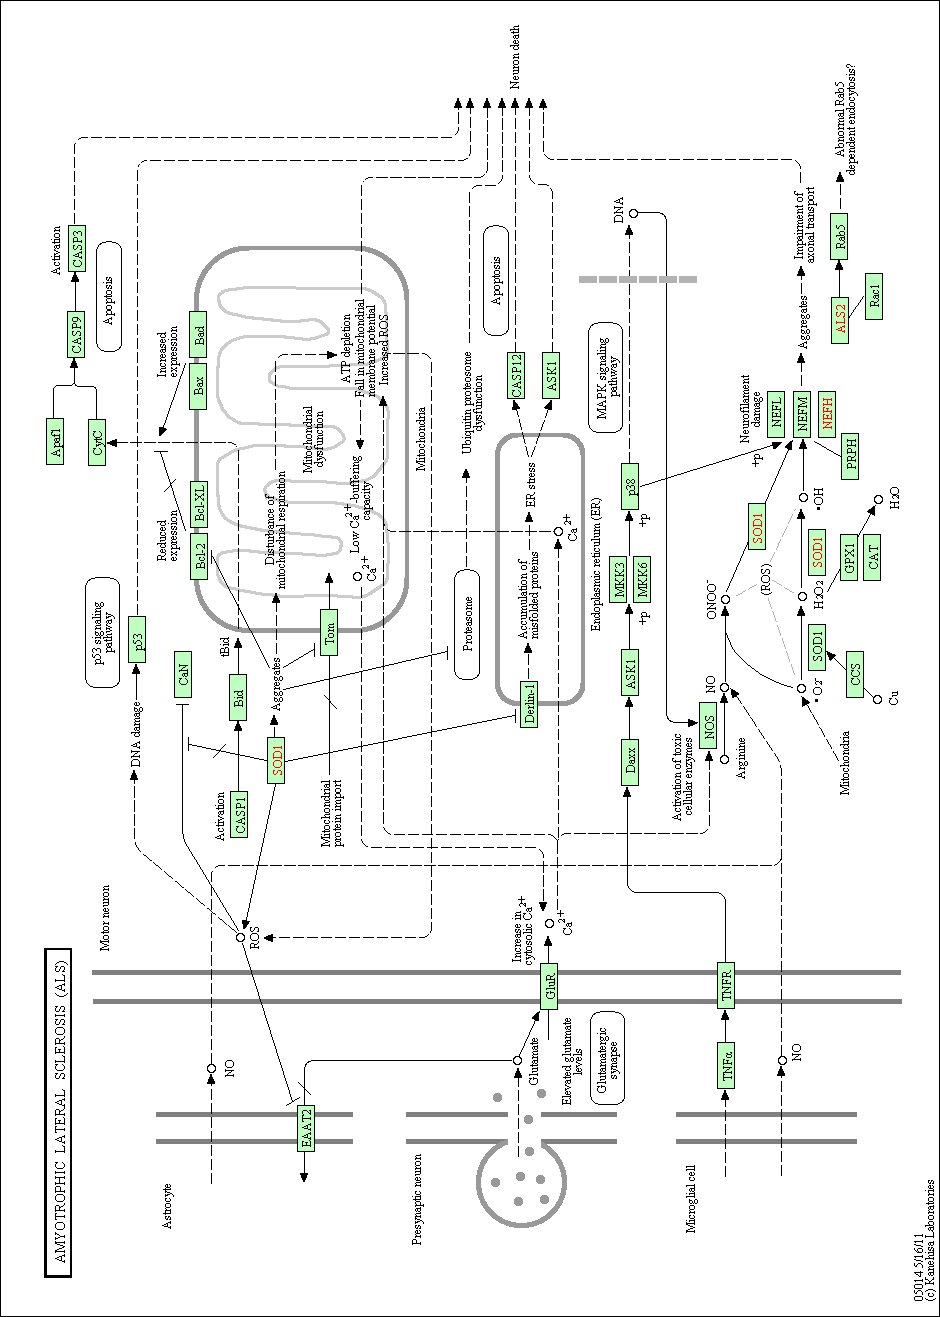
\includegraphics[width=\textwidth]{mmu05014_cl197_Potrait.png}
\caption {Pathway analysis: KEGG\_Pathway. \label{pathwayAnalysis}}
 \end{center}
\end{figure}
Pathway analysis allows us to gain an insight of the underlying biology of the differentially expressed genes. Pathway analysis can reduce the complexity and increase the explanatory power where high-throughput sequencing and gene profiling are used to investigate whether a gene or a list of gene have any roles for a phenotype or a given phenomena. It is also used for the analysis of gene ontology, physical interaction networks, inference of pathways from expression and sequence data, and further comparisons. In a given condition it can identify the pathway by correlating information with a pathway knowledge base. We identified some clusters (which were deemed interesting in the cluster analysis and enrichment score analysis stages) and performed gene ontology enrichment analysis (one example is given at Table \ref{table:funAnno}) and pathway analysis on individual clusters.  We identified one of our cluster (cluster197; Figure \ref{fig:fourSampleClusters}) which was selected at the earlier stage for further analysis and has a relatively high enrichment score (2.16) is related with ALS.  In previous study \cite{Brockington:2013} reported about $SOD1$ related genes and ALS.  One of the $SOD1$ gene, $Derlin-1$ (Prob ID: 1415693_at), can accumulate with other misfolded proteins and cause the neuron death and belongs to our chosen cluster. Figure \ref{pathwayAnalysis} shows the pathway analysis that we have found for one of our cluster using tool $DAVID$.  We have also found some other genes from the same cluster are responsible for cell death and related with some other neural disorder. 

\begin{figure}
 \begin{center}
 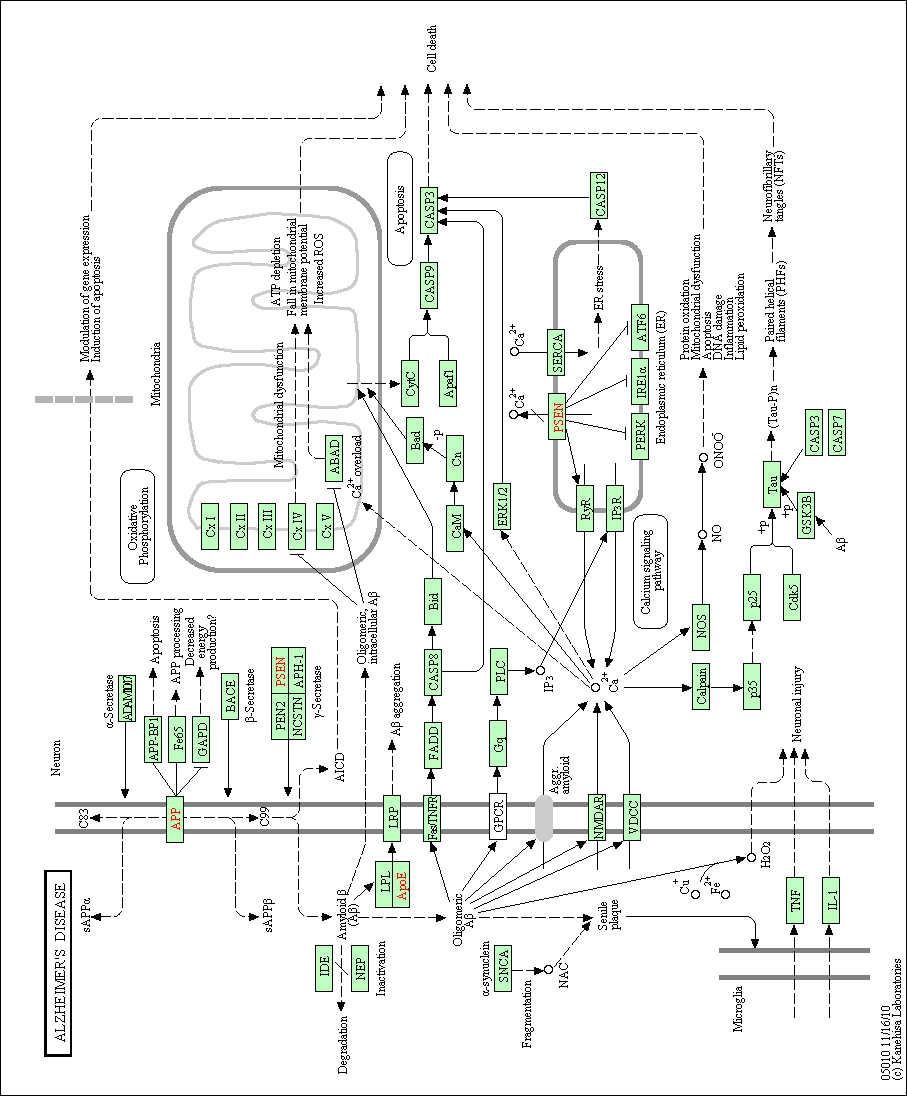
\includegraphics[width=\textwidth]{Alzheimers_mmu05010.png}
\caption {KEGG\_Pathway analysis of Alzheimer's disease. \label{AlzheimerPathwayAnalysis}}
 \end{center}
\end{figure}


\begin{figure}
 \begin{center}
 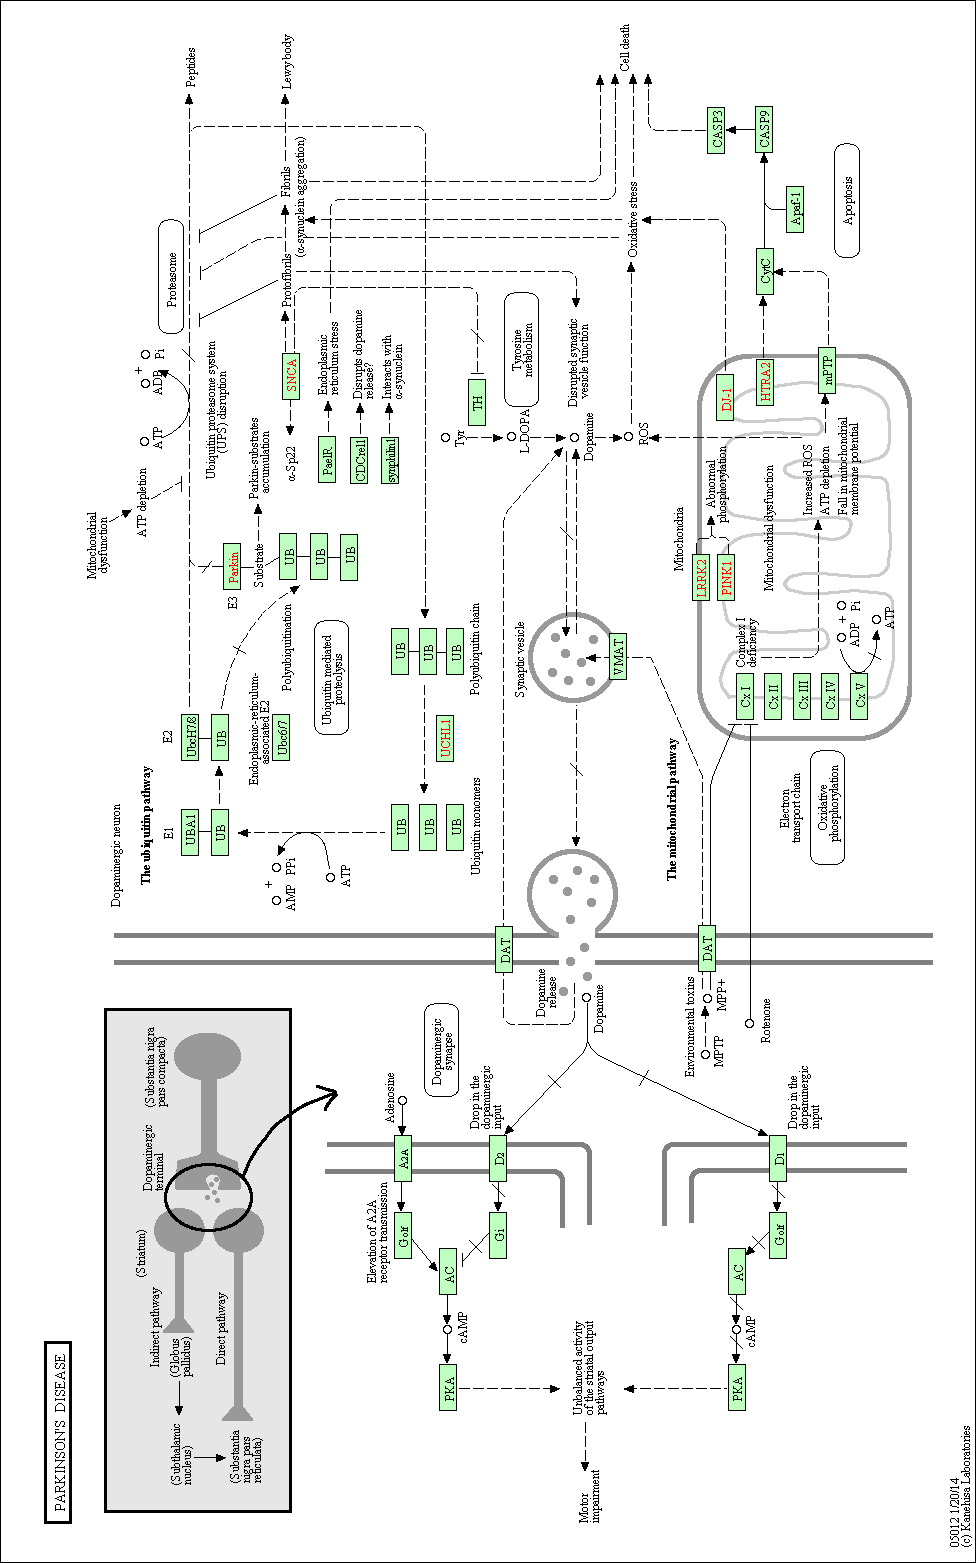
\includegraphics[width=\textwidth]{Parkinsons_mmu05012.png}
\caption {KEGG\_Pathway analysis of Parkinson's disease. \label{ParkinsonPathwayAnalysis}}
 \end{center}
\end{figure}


\section{Discussion}
We have performed genome-wide analysis to cluster genes systematically and analyse the rationale behind the variation in the speed of propagation for ALS. Our particular innovation was to include the condition and genetic background of the organisms within the underlying functional component of our clusters. This ensured that sub-groups where the underlying expression behaved similarly were more likely to cluster together. The hierarchical Gaussian process we used considers multiple replicates. For validation we have used a widely acceptable gene ontology and functional annotation tool to validate our clusters and their characteristics obtained from our model. We found a number of clusters are highly enriched. Gene expression time series characteristics curve and enrichment scores analyse helped us to narrow down our search and lead toward finding the lists of genes or clusters which could be involved in the speed of disease propagation. Our pathway analysis found a gene which is known to be
involved in the disease process. Here we started with whole genome set and ended with a single gene. This finding lead us to conclude that the model we have developed based on Gaussian process can cluster the genes successfully and they are very much informative. These clusters can be useful for further analysis.  Even the model we have developed using hierarchical Gaussian process could be useful to investigate other biological activity where clustering is required. 
